%\pdfminorversion=7
\documentclass[a4paper,12pt]{report} % Foglio a4, font size 12, solo fronte


\usepackage[utf8]{inputenc} % Codifica caratteri
\usepackage[T1]{fontenc}
\usepackage[includehead, inner=3.0cm, outer=2.0cm, top=2.5cm, bottom=2.5cm]{geometry}
\usepackage{charter} % Text font
\usepackage[titles]{tocloft} % TOC compatta
\usepackage{amssymb} % Checkmark e altri simboli
\usepackage{graphicx} % Per inserire immagini
\usepackage{float} % Per controllare il posizionamento di immagini e tabelle
\usepackage[bottom]{footmisc} % Footer in fondo alla pagina
\usepackage[section]{placeins} % Force all floats before section end

\usepackage[english,italian]{babel}
\usepackage{amsmath, caption}
\usepackage[skip=8pt]{parskip}

\usepackage{listings}
\renewcommand{\lstlistingname}{Listato}
\usepackage{xcolor}
\usepackage{setspace}
\usepackage{csquotes}
\usepackage[
backend=biber,
style=apa,
sorting=ynt,
uniquelist=false]{biblatex}
\addbibresource{bibliography.bib} % Bibliografia su un file a parte
%\addbibresource{refs.bib} % File contentente la bibliografia


\let\Chapter\chapter\def\chapter{\addtocontents{lol}{\protect\addvspace{10pt}}\Chapter}

% Glossary
\usepackage[acronym,nonumberlist]{glossaries}
%\makeglossaries

% Liste
\usepackage{enumitem} % Per inserire liste
\usepackage{siunitx} % Per usare \setitemize
\setitemize{noitemsep,topsep=0pt,parsep=0pt,partopsep=0pt} % itemize più compatto
\setenumerate{noitemsep,topsep=0pt,parsep=0pt,partopsep=0pt} % enumerate più compatto
\setenumerate{noitemsep,topsep=0pt,parsep=0pt,partopsep=0pt} % enumerate più compatto
\setdescription{topsep=0pt} % enumerate più compatto

% Captions
\usepackage[font=small,textformat=period]{caption}
\captionsetup{justification=centering}

% Numerazione enumerate innestati
\renewcommand{\labelenumii}{\theenumii}
\renewcommand{\theenumii}{\theenumi.\arabic{enumii}.}

% Spaziature
\linespread{1.5} % Interlinea
\setlength{\parindent}{6pt} 
\setlength{\parskip}{1em} % Spazio tra paragrafi
\setlength{\headheight}{15pt} % Risolve warning con fancyhdr

% Formato capitoli
\usepackage{titlesec}
\titleformat{\chapter}[hang]{\normalfont\Huge\bfseries}{\thechapter.}{8pt}{\Huge\bfseries}
\titleformat*{\section}{\LARGE\bfseries}
\titleformat*{\subsection}{\Large\bfseries}
\titleformat*{\subsubsection}{\large\bfseries}
\titlespacing*{\chapter}{0pt}{-40pt}{15pt}
\titlespacing*{\section}{0pt}{18pt}{8pt}
\titlespacing*{\subsection}{0pt}{14pt}{6pt}
\titlespacing*{\subsubsection}{0pt}{10pt}{4pt}

% Intestazione pagine
\usepackage{fancyhdr}
\pagestyle{fancy}
\renewcommand{\chaptermark}[1]{\markboth{\thechapter. #1}{#1}}
\fancyhf{}
\fancyhead[L]{\small\slshape\nouppercase{\leftmark}}
\fancyfoot[C]{\thepage}
\renewcommand{\headrulewidth}{0.4pt}


\makeatletter
\renewcommand\paragraph{%
  \@startsection{paragraph}
    {4}
    {\z@}
    {3.25ex \@plus1ex \@minus.2ex}
    {-1em}
    {\normalfont\normalsize\bfseries\maybe@addperiod}%
}
\newcommand{\maybe@addperiod}[1]{%
  #1\@addpunct{.}%
}
\makeatother

\newcommand{\figura}[4]{%
  \begin{figure}[htbp]
    \centering
    \includegraphics[width=#1\textwidth]{#2}
    \caption{#3}\label{#4}
  \end{figure}%
}


% URL
\usepackage[hidelinks]{hyperref} % Per inserire URL
\usepackage{hyperxmp}


\newacronym{tpm}{TPM}{Trusted Processing Modules}
\newacronym{tc}{TC}{Trusted Computing}
\newacronym{pc}{PC}{Personal Computers}
\newacronym{rot}{RoT}{Root of Trust}
\newacronym{drm}{DRM}{Digital Rights Management}
\newacronym{hmac}{HMAC}{Keyed-Hash Message Authentication Code}
\newacronym{mac}{MAC}{Message Authentication Code}
\newacronym{ca}{CA}{Certificate Authority}
\newacronym{pki}{PKI}{Public Key Infrastructure}
\newacronym{pcr}{PCR}{Platform Configuration Register}
\newacronym{cpu}{CPU}{Central Processing Unit}
\newacronym{tcg}{TCG}{Trusted Computing Group}
\newacronym{tss}{TSS}{TPM Software Stack}
\newacronym{api}{API}{API}
\newacronym{so}{SO}{Sistemi Operativi}
\newacronym{fapi}{FAPI}{Feature API}
\newacronym{esapi}{ESAPI}{Enanched System API}
\newacronym{sapi}{SAPI}{System API}
\newacronym{tcti}{TCTI}{TPM Command Transmission Interface}
\newacronym{rm}{RM}{Resource Manager}
\newacronym{tab}{TAB}{TPM Access Broker}
\newacronym{dd}{DD}{Device Driver}
\newacronym{crb}{CRB}{Command Response Buffer}
\newacronym{pin}{PIN}{PIN}
\newacronym{vmk}{VMK}{VMK}
\newacronym{fvek}{FVEK}{FVEK}
\newacronym{xts}{XIS}{XTS}
\newacronym{aes}{AES}{AES}
\newacronym{amd}{AMD}{AMD}
\newacronym{elam}{ELAM}{Early Launch Anti-Malware}
\newacronym{ccp}{CCP}{Crypto Co-Processor}
\newacronym{smn}{SMN}{Secure Memory Network}
\newacronym{dtpm}{dTPM}{Discrete Trusted Platform Module}
\newacronym{ftpm}{fTPM}{Firmware Trusted Platform Module}
\newacronym{dram}{DRAM}{Dynamic Random-Access Memory}
\newacronym{sev}{SEV}{Secure Encrypted Virtualization}
\newacronym{vbs}{VBS}{Virtualization-Based Security}
\newacronym{rng}{RNG}{Random Number Generator}
\newacronym{iot}{IoT}{Internet of Things}
\newacronym{arm}{ARM}{Advanced RISC Machines}
\newacronym{sw}{SW}{Secure World}
\newacronym{nw}{NW}{Normal World}
\newacronym{soc}{SoC}{System on Chip}
\newacronym{io}{I/O}{Input/Output}
\newacronym{rpmb}{RPMB}{Replay Protected Memory Block}
\newacronym{tee}{TEE}{Trusted Execution Environment}
\newacronym{rsa}{RSA}{Rivest-Shamir-Adleman}
\newacronym{txt}{TXT}{Trusted Execution Technology}
\newacronym{drtm}{DRTM}{Dynamic Root of Trust for Measurement}
\newacronym{tcb}{TCB}{Trusted Computing Base}
\newacronym{acm}{ACM}{Authenticated Code Module}
\newacronym{dma}{DMA}{Direct Memory Access}
\newacronym{psp}{PSP}{Platform Security Processor}
\newacronym{nv}{NV}{Non-Volatile}

\newacronym{hsm}{HSM}{Hardware Security Module}
\newacronym{ssl}{SSL}{Secure Sockets Layer}
\newacronym{tls}{TLS}{Transport Layer Security}
\newacronym{srk}{SRK}{Storage Root Key}
\newacronym{spi}{SPI}{Serial Peripheral Interface}
\newacronym{tpme}{TPME}{TPM Enablement}
\newacronym{ek}{EK}{Endorsement Key}
\newacronym{ai}{AI}{Intelligenza Artificiale}
\begin{document}

% PDF metadata
\hypersetup{
  bookmarksopen=true,
  pdftitle={Trusted Processing Modules: Storia, Evoluzione e Applicazioni},
  pdfauthor={Wade Giovanni Baisini}}

% Info documento
\title{Trusted Processing Modules: Storia, Evoluzione e Applicazioni}
\author{Wade Giovanni Baisini}
\date{March 2025}

\newgeometry{lmargin=2cm,rmargin=2cm,tmargin=2.5cm,bmargin=2cm} % Bordi pagina come da formato tesi Unibs
\begin{titlepage}
    \begin{center}
    \begin{spacing}{1.5}
    \vspace{25mm}
    
\includegraphics[]{figures/frontespizio.png}\\
    \vspace{13mm}
    {{\Large{\textsc{DIPARTIMENTO DI INGEGNERIA DELL'INFORMAZIONE}}}}\\
    {\large{\it Corso di Laurea \\in Ingegneria Informatica}}
    \end{spacing}
    \end{center}
    \begin{center}
    \begin{spacing}{1.5}
        
    {\large Tesi di Laurea}
    
    {\LARGE{\textsc{Trusted Processing Modules: \\storia, evoluzione e applicazioni}}}\\
    
    \end{spacing}
    \end{center}
    \vspace{25mm}
    \par
    \noindent
   
    
    \begin{minipage}[t]{0.47\textwidth}
                \raggedright
                \textbf{Relatore:} \\[0.3em]
                Chiar.mo Prof. Giuzzi Luca \\[1em]
            \end{minipage}
            \hfill
            \begin{minipage}[t]{0.47\textwidth}\raggedleft
                \textbf{Laureando:} \\[0.3em]
                Wade Giovanni Baisini \\
                \text{Matricola 735655}
            \end{minipage}
            \vfill
    
    \vspace{25mm}
    \begin{center}
    %\vfill
    {\large{\it Anno Accademico 2023/2024 }}
    
    \end{center}
    \end{titlepage}
\restoregeometry

\clearpage
\thispagestyle{empty} % Rimuove numero di pagina e intestazioni per questa pagina

\vspace*{\fill} % Spinge il testo verticalmente verso il centro-basso della pagina

\begin{flushright}
  \itshape 
Ma la verità è che la tecnologia\\
è molto politica  \- nel modo\\
in cui viene creata, sviluppata,\\ 
da chi, per chi e perché\\
\end{flushright}

\vfill
\clearpage

\hyphenpenalty=2000
\textwidth=450pt\oddsidemargin=0pt

\pagenumbering{Roman}
\tableofcontents
\cleardoublepage
\pagenumbering{arabic}

% inserisci i file contenenti le sezioni
\chapter*{Introduzione}\label{ch:introduzione}
\markboth{Introduzione}{Introduzione}
\addcontentsline{toc}{section}{Introduzione}

Negli ultimi anni si sono sensibilmente espansi il dibattito e la ricerca attorno la tecnologia del \acrfull{tc}.
Con la digitalizzazione della maggior parte dei momenti della nostra vita, diventa essenziale prevedere meccanismi e garanzie di sicurezza, confidenzialità e integrità anche in ambienti informatici.
Trusted Computing -- "calcolo fidato -- si riferisce ad un tipo di tecnologia che ha l’obiettivo di garantire che dei dispositivi (come computer o telefoni cellulari) siano protetti da eventuali manomissioni come l’iniezione di codici estranei, mediante l’uso di opportuni hardware e software.
Data l’incredibile varietà del software e degli algoritmi, delle applicazioni e delle tecnologie hardware, è fondamentale che esista un metodo di riferimento per garantire affidabilità in questo settore. Ricordando è doveroso rimanere sempre consapevoli che al giorno d’oggi non esiste un meccanismo per trasformare uno standard dalla sua specifica all’implementazione in maniera impeccabile: anzi il processo di implementazione è il momento più rischioso e delicato. Un’implementazione che sarebbe altresì perfetta -- di un crittosistema perfetto, crollerebbe se esistesse anche solo un piccolo dettaglio implementativo che fornisca \enquote{backdoor} o \enquote{scorciatoie} di qualsiasi natura.  
Questo testo cerca di navigare una questione molto ampia delineando prima il problema di sicurezza in analisi, e poi una soluzione particolare ad una piattaforma. Nel dettaglio si tratterà di \acrfull{tpm} -- da qui in poi \acrshort{tpm} -- la specifica e proposte di implementazione “ufficiali”. 
Il \acrshort{tpm} è una soluzione che viene ideata in primissimo luogo pensando ai calcolatori personali, ai \acrfull{pc}, ma verranno citate anche proposte che spaziano su tutt’altro tipo di hardware, trasformandosi talvolta in soluzioni diverse allo stesso problema.

\chapter{Il problema}\label{ch:il_problema}

\section{Perché serve il Trusted Computing?}\label{sec:perche_tc}
Come già analizzato nell'introduzione di questo testo, uno dei problemi più rilevanti nel campo delle applicazioni sicure è la protezione della piattaforma hardware contro attacchi alla sua integrità o modifiche del codice sicuro.

Sebbene le soluzioni software possano fornire una certa protezione, sono certamente limitate dall'incapacità di presentare all'utente un ambiente di esecuzione che possa essere separato in modo efficace dalla realtà fisica. Tecniche come l'emulazione o l'intercettazione delle operazioni (ad esempio, la modalità SMI delle CPU) non possono garantire la protezione intrinseca necessaria in scenari di alta sicurezza. 

Un ulteriore aspetto importante riguarda i segreti memorizzati e utilizzati dai dispositivi, come chiavi private essenziali per l'autenticazione o certificati digitali. Non è necessario che questi dati vengano trattati direttamente a livello software, ma piuttosto tramite informazioni derivate da essi. La loro protezione è cruciale, non solo per salvaguardare l'accesso ai servizi e alle risorse sensibili, ma anche per prevenire che il sistema operativo o altre applicazioni possano compromettere l'integrità dei dati. Per tale motivo, la protezione hardware di questi segreti diventa fondamentale, poiché garantisce che i segreti restino sicuri anche in caso di attacchi software senza mai esporli in chiaro, nemmeno al sistema operativo stesso.

Nell'ambito dei \acrshort{pc} (o dei dispositivi in generale) gli attacchi e gli incidenti più noti sono quelli che riguardano l'\textit{home banking}, ma esistono anche attacchi rivolti ai server utilizzati dalle aziende per fornire servizi e trattare dati sensibili. Purtroppo, i rischi si estendono anche ad altri tipi di piattaforme, come i sistemi \textit{embedded}, che sono spesso meno protetti. Esempi tipici di queste vulnerabilità sono la manipolazione dei dati e del codice presenti su controller \textit{automotive}, sistemi antifurto delle auto o sistemi di domotica.

Fino a oggi tutti i tentativi di risoluzione che affrontano il problema da un punto di vista puramente software non hanno trovato conclusioni incoraggianti. Come ci insegna l'esperienza e la storia del mondo delle \textit{smart card}, una base di sicurezza fidata e a prova di manomissione non può essere implementata usando solo soluzioni software. Questo approccio si applica sia alle piattaforme \acrshort{pc} sia a quelle \textit{embedded}. Per questo motivo è indispensabile avere un ancoraggio hardware, un componente fidato che possa fungere da base per costruire una catena di fiducia in grado di resistere a tentativi di manipolazione. Il concetto verrà approfondito nella sezione dedicata alla \enquote{Root of Trust}.

Il mondo informatico si è accorto della necessità di sistemi di sicurezza ancorati sull'hardware per diverse ragioni e in momenti specifici. Principalmente negli anni '90, quando inizia a diffondersi Internet, l'industria si spostò \textit{online} e questo implicò una necessità di sicurezza anche nel \textit{cloud}: questa necessità venne sottolineata velocemente dai diversi e nuovi attacchi \textit{malware} sempre più sofisticati.

Fino a quel momento il mezzo principale per difendersi dai \textit{malware} erano gli antivirus. Ma il difetto fondamentale di un approccio di difesa basato esclusivamente sul software è che il software non può verificare efficacemente sé stesso. Se un \textit{malware} ottiene l'esecuzione con lo stesso livello di privilegio del software antivirus, può semplicemente disabilitarlo e nascondersi dagli \enquote{occhi} del sistema operativo. In quegli anni gli attacchi informatici iniziarono a prendere di mira anche il \textit{firmware} e il codice del \textit{bootloader}, che raramente vengono verificati dal software antivirus. 

In secondo luogo si espande l' \textit{e-commerce}, che porta a un aumento ingente di transazioni finanziarie \textit{online}. Diventa critica la presenza di un'infrastruttura per permettere alle banche e altre istituzioni di supportare questo nuovo mercato, ma soprattutto di permettere agli utenti di accedere ai servizi (come l'\textit{home banking}) in maniera segreta, protetta e sicura.

Per verificare in modo sicuro la configurazione del software, una piattaforma di calcolo ha bisogno di un luogo per registrare e verificare lo stato del software che sia esterno allo spazio di memoria principale del sistema. Questo concetto si chiama \enquote{monitor di sicurezza hardware}.

Il \acrshort{tc} è l'implementazione tecnologica di tecniche che già sono utilizzate ogni giorno per stabilire legami di fiducia tra persone. Questa soluzione tecnologica è progettata per trasformare ogni piattaforma in un ambiente sicuro: ovvero deve esistere un metodo per isolare efficacemente determinati dati e applicazioni dal \enquote{resto del mondo}. 

La tecnologia di \acrshort{tc} è progettata affinché la piattaforma non possa mentire né travisare, nemmeno se l'utente desidera farlo: elemento essenziale, poiché nessuno può fidarsi di una piattaforma che offre tale possibilità. Questa tecnologia cerca di garantire che gli utenti che si espongono a rischi lo facciano tramite una scelta consapevole. Il \acrshort{tc} include metodi progettati per proteggere gli interessi degli utenti, mantenendo la loro \textit{privacy}, e per assicurare che possano continuare a fare \textit{backup} e recuperare i dati. I programmi software e gli utenti devono scegliere deliberatamente di ignorare i suggerimenti della tecnologia se vogliono creare dati che non possano essere recuperati.

Una piattaforma può garantire l'affidabilità dei suoi componenti solo se si fonda su meccanismi di fiducia sicuri. In questo contesto, le \textit{Root of Trust} svolgono un ruolo cruciale: costituiscono il fondamento su cui si costruisce la sicurezza di una piattaforma, in quanto assicurano che ogni operazione venga eseguita correttamente e senza alterazioni. Se una \textit{Root of Trust} viene compromessa, disabilitata o alterata, la piattaforma perde la sua capacità di essere sicura.


\section{Root of Trust}\label{sec:root_of_trust}
La \acrfull{rot} è una componente di sicurezza essenziale e fondamentale che fornisce un insieme di funzioni affidabili, utilizzabili dal resto del dispositivo o sistema per stabilire meccanismi e livelli di sicurezza elevati. 

La \acrshort{rot} è spesso integrata come un chip e costituisce una fonte di fiducia fondamentale per qualsiasi sistema crittografico. Quando si parla di \acrshort{rot} come un chip, allora lo si può indicare come un \textit{Hardware Root of Trust} (H-RoT). Richiedendo che la \acrshort{rot} sia intrinsecamente affidabile, deve essere sicura per definizione. Per questo la forma di implementazione più sicura è in hardware, in quanto diventa immune agli attacchi \textit{malware}. Operativamente può essere un modulo di sicurezza autonomo o implementato come modulo di sicurezza all'interno di un processore o di un \textit{System on Chip} (SoC).

Le funzioni principali di una \acrshort{rot} includono il \textit{boot} sicuro, la misurazione, la memorizzazione sicura, la segnalazione e la verifica, con la capacità di conservare le chiavi crittografiche riservate al di fuori del software di sistema, che è frequentemente mirato dagli attaccanti. 

Il concetto di \textit{boot} sicuro prevede di instaurare una catena di fiducia necessaria per garantire un processo di avvio sicuro e con codice legittimo. Se il primo pezzo di codice è stato verificato positivamente, allora le credenziali associate con l'accesso a quel codice vengono poi considerate come fidate nell'esecuzione di ogni pezzo successivo. In altre parole, le \acrshort{rot} permettono a una piattaforma di dimostrare che è un ambiente protetto, rilasciando i dati protetti solo dopo che il software in esecuzione è stato verificato come sicuro: software sicuro e piattaforma hardware fidata sono gli ingredienti per un ambiente protetto. 

A titolo aggiuntivo si nota che il \acrshort{tc} non è sempre ben visto nell'immaginario comune (uscendo da quello strettamente tecnico) poiché legato anche a tecniche di \acrfull{drm}. Il \acrshort{drm} viene usato per controllare l'accesso ai contenuti digitali e per impedire azioni che violino i diritti d'autore, di fatto imponendo restrizioni sulle operazioni che gli utenti possono effettuare sui contenuti digitali (ad esempio l'esecuzione esclusiva di applicazioni firmate, la richiesta di licenze per determinati contenuti o il vincolo di file multimediali a una specifica macchina). Si sottolinea che questo è solo uno dei possibili utilizzi, nonostante sia uno dei più pubblicamente controversi.


\section{Ipotesi e considerazioni}\label{sec:ipotesi_considerazioni}
Per poter parlare di una tecnologia come il \acrshort{tpm}, bisogna essere consapevoli che è solo una delle possibili soluzioni a un problema più ampio. A questo fine si delineano i concetti principali per descrivere le problematiche a cui si vorrebbe far fronte.

Come prima assunzione, è necessario immaginare di prendere in esame un modello che preveda attacchi ragionevoli e non hardware. Questo perché si vorrebbe calarsi in un mondo -- non ideale -- che approssima al meglio possibile le reali relazioni di potere e rischio che sussistono tra utenti e fornitori di servizi (intesi come entità hardware, software o attori dell'industria informatica).

Per attacchi ragionevoli si intende una situazione nella quale l'utente comune non è vittima di attacchi mirati da parte di agenti che possiedono risorse e capacità di calcolo rasenti al massimo dello stato corrente dell'arte. Verranno citate per completezza e consapevolezza anche casistiche in cui la posta in gioco è maggiore, come ambienti in cui gli attori sono entità del calibro di organizzazioni governative.

Per attacchi non hardware si intende escludere la possibilità che l'agente attaccante abbia accesso fisico illimitato al dispositivo e che questo non sia compromesso a prescindere. Il problema della sicurezza intesa come accesso fisico a una macchina è un problema diverso, ma è anche il dilemma più vecchio: prima dell'avvento delle reti di interconnessione tra calcolatori, l'unico modo per interagire con una macchina implicava la presenza fisica dell'operatore. 

Questo tipo di problema trova sicuramente spazio anche oggigiorno, ma l'ambito di questo testo vuole analizzare alcune soluzioni a questioni che non ammettono l'ipotesi di una piattaforma già compromessa. Se il dispositivo personale di un utente non è affidabile, allora qualsiasi sistema per la protezione di credenziali e dati utente che deve essere utilizzato su quest'ultimo risulterebbe inutile, poiché non esisterebbe una base sicura.

Per fare una sintesi, assumiamo che:
\begin{itemize}
    \item l'attaccante sia non-onnipotente;
    \item i dispositivi non siano compromessi prima dell'applicazione delle soluzioni;
    \item i dispositivi non siano fisicamente disponibili all'attaccante in maniera incontrollata.
\end{itemize}

Quello che si vuole analizzare principalmente sono le soluzioni per:
\begin{enumerate}
    \item garantire l'accesso sicuro alle credenziali di autenticazione;
    \item verificare il software del sistema operativo, indipendentemente dallo stesso, per contrastare possibili condotte malevole verso la CPU.
\end{enumerate}

Il \acrshort{tpm} offre strumenti per lavorare verso l'ottenimento di queste condizioni, tant'è che fin dalla prima specifica viene esplicitato che la sicurezza dell'ambiente fisico di esecuzione non è definita e che sarà compito dei singoli produttori occuparsene. È importante ribadire che questo tipo di sicurezza è un problema che sta a monte rispetto a quello di garantire credenziali sicure. 


\section{Elementi essenziali di crittografia}\label{sec:crittografia}
Di seguito vengono elencate alcune nozioni essenziali per poter comprendere quanto trattato.

\subsection{Algoritmi crittografici}\label{subsec:algoritmi_crittografici}
Il cuore di un sistema crittografico sono in generale gli algoritmi crittografici di cui questo fa uso. Un algoritmo crittografico prende un input (come un messaggio) e lo trasforma tramite funzioni matematiche e una chiave che controlla queste funzioni per produrre un singolo output.

Le operazioni di cifratura utilizzano la chiave crittografica per trasformare il messaggio originale in una forma crittografata. La decifratura fa l'opposto: usa una chiave crittografica per trasformare un messaggio crittografato nel suo formato originale (detto anche testo in chiaro). 

Una chiave è semplicemente un numero o una sequenza di bit. Si vorrebbe usare una chiave sufficientemente grande in modo che non possa essere indovinata o scoperta con tentativi sistematici. La lunghezza di questa chiave dipende dal tipo di algoritmo e da quanto il sistema deve essere sicuro (ad esempio, oggi sono molto usate le chiavi RSA a $2048$ bit, ma lo standard si sta spostando verso i $3072$ bit).

Esistono due grandi famiglie di algoritmi crittografici, che differiscono per il numero e i tipi di chiavi utilizzate: algoritmi simmetrici e algoritmi asimmetrici.

\subsubsection{Algoritmi simmetrici}\label{subsubsec:algoritmi_simmetrici}
Gli algoritmi simmetrici utilizzano la stessa chiave per la cifratura e la decifratura. La forza di un algoritmo simmetrico dipende dalla dimensione della chiave, con la sicurezza che cresce esponenzialmente con il numero di bit. La chiave deve essere nota al mittente e al destinatario prima della comunicazione sicura.

\subsubsection{Algoritmi asimmetrici o a chiave pubblica}\label{subsubsec:algoritmi_asimmetrici}
Negli algoritmi asimmetrici le operazioni di cifratura e decifratura sono differenti e utilizzano chiavi differenti. Insieme le chiavi formano una coppia detta coppia di chiavi pubblica e privata. 

Il destinatario di un messaggio rende pubblica la propria chiave pubblica e conserva la chiave privata. Per comunicare è sufficiente utilizzare la sua chiave pubblica per cifrare il messaggio. Così facendo la decifratura -- per definizione dell'algoritmo -- può essere effettuata solo con la chiave privata. Se qualcuno intercetta il messaggio lungo il tragitto, non sarà in grado di leggerlo senza accesso alla chiave privata.

Il principale vantaggio rispetto agli algoritmi simmetrici è che non è necessario scambiare la chiave in modo sicuro prima di iniziare la comunicazione, rendendo così il sistema molto più semplice da gestire e utilizzare. La chiave pubblica può essere nota a chiunque senza che questo rappresenti un rischio, a patto che la chiave privata sia davvero nota solo al suo proprietario.


\subsection{Funzioni di hashing}\label{subsec:funzioni_hashing}
Le funzioni di \textit{hashing} sono invece sfruttate per garantire l'integrità dei messaggi trasmessi tra le parti che comunicano. L'integrità fornisce la certezza che il messaggio non sia stato manomesso. I meccanismi di \textit{hashing} sono utilizzati anche per firmare digitalmente i dati.

Una funzione di \textit{hash} sicura è come un algoritmo che può cifrare ma non decifrare: in altre parole, dato un input è possibile calcolare un output, ma dato un output (messaggio cifrato) non è possibile risalire all'input (messaggio in chiaro). Due proprietà importanti di queste funzioni sono:
\begin{enumerate}
    \item Dallo stesso input si ottiene sempre la stessa stringa in output.
    \item Indipendentemente dall'input o dalla sua lunghezza, l'output ha sempre la stessa dimensione.
\end{enumerate}

Il mittente genera il messaggio insieme a un \enquote{digest}, ovvero utilizza il messaggio come input alla funzione di \textit{hashing}. Il \enquote{digest} di un messaggio può essere inteso come un suo \enquote{riepilogo}. Il messaggio cifrato è poi spedito insieme al \enquote{digest}, in modo tale che il destinatario possa decifrare il messaggio e inserirlo nella stessa funzione di \textit{hash}. Se i due \enquote{digest} (quello ricevuto e quello calcolato) coincidono, allora il messaggio è originale. 


\subsubsection{Hash Extend}\label{subsubsec:hash_extend}
La funzione di \textit{extend} di un \textit{hash} non è comune nella crittografia in generale, ma è fondamentale per alcune attività del \acrshort{tpm}. 

L'operazione di \textit{extend} inizia con un valore di input $A$ a cui viene concatenato un altro valore $B$ (il valore che deve essere esteso), ottenendo la stringa $A \mathbin{\Vert} B$. Successivamente, si applica la funzione di \textit{hash} a questa unione e il risultato andrà a rimpiazzare il vecchio valore $A$:
\begin{equation}\label{eq:hash_extend}
    A_{\text{new}} = \operatorname{hash}(A_{\text{old}} \mathbin{\Vert} B)
\end{equation}

Grazie alle proprietà di \textit{hashing} sicuro, diventa impossibile ripristinare un valore \textit{hash} esteso al suo valore precedente, permettendo al \acrshort{tpm} di mantenere uno \enquote{storico} delle modifiche e delle misurazioni.


\subsubsection{HMAC}\label{subsubsec:hmac}
Un \acrfull{hmac} è una funzione di \textit{hash} che utilizza una chiave segreta per generare un \acrfull{mac} univoco. Questo \acrshort{mac} è utile per firmare dati o autenticare entità, oltre che per garantire l'integrità grazie alle proprietà di \textit{secure hash}.

Il destinatario riceve il \acrshort{mac} calcolato dal mittente usando la chiave condivisa e la stessa funzione di \textit{hash}. Se il \acrshort{mac} calcolato dal destinatario è uguale a quello trasmesso, allora il messaggio è integro; inoltre, siccome è stata necessaria una chiave condivisa, il mittente è anche autenticato agli occhi del destinatario.


\subsection{Certificati digitali}\label{subsec:certificati_digitali}
Un certificato digitale è un documento elettronico che associa una chiave pubblica a un'entità, come una persona o un'organizzazione, e ne attesta l'autenticità attraverso la firma digitale di una terza parte fidata, chiamata \acrfull{ca}. I certificati sono utilizzati principalmente per garantire la sicurezza delle comunicazioni in sistemi crittografici asimmetrici, in cui la chiave pubblica deve essere affidabile. 

Essi permettono di stabilire la fiducia tra soggetti che non si conoscono direttamente, in modo tale che non debbano scambiarsi le chiavi pubbliche prima della comunicazione: possono \enquote{semplicemente fidarsi} che, se la chiave è firmata da una \acrshort{ca} attendibile, allora anche l'entità con cui stanno per parlare è attendibile. 

L'infrastruttura che gestisce questi certificati è conosciuta come \acrfull{pki}. La \acrshort{pki} garantisce la validità e l'integrità del certificato attraverso un processo di verifica dell'identità del richiedente, svolto dalla \acrshort{ca} stessa.
\chapter{Modello di attacco}\label{ch:modello_attacco}

Uscendo temporaneamente dal contesto della sicurezza hardware, è opportuno approfondire la natura delle minacce da cui ci si intende proteggere e definire rigorosamente cosa si intenda per \enquote{sistema sicuro}.

\begin{quote}
    \enquote{I sistemi di sicurezza che utilizzano la crittografia sono progettati per impedire alle persone malintenzionate di manipolare i tuoi dati, impersonare te o modificare documenti senza essere rilevati.}
\end{quote}

Questa affermazione può essere un buon punto di partenza se si cercasse un principio fondamentale da non dimenticare mai. Tuttavia, la sua semplicità rischia di far trascurare l'intrinseca complessità dei sistemi di sicurezza e di quelli che gestiscono informazioni più in generale. 

Durante lo studio di soluzioni reali, tuttavia, diventa necessario compiere un salto logico dalla teoria alla pratica. Possiamo facilitare questo passaggio fornendo alcune definizioni operative: affermiamo che la crittografia è l'arte di comunicare in presenza di avversari, sfruttando operazioni, proprietà e problemi matematici. 


\section{I requisiti della sicurezza informatica}\label{sec:requisiti_sicurezza}
La sicurezza della comunicazione si basa tradizionalmente su quattro requisiti fondamentali:
\begin{itemize}
    \item \textbf{Confidenzialità:} il messaggio, ossia il contenuto della comunicazione, deve rimanere segreto e intellegibile solo al legittimo mittente e al destinatario autorizzato.
    \item \textbf{Integrità:} le informazioni non devono poter essere modificate durante l'archiviazione o il transito. Qualora ciò avvenga, la modifica deve essere rilevata tempestivamente.
    \item \textbf{Autenticazione:} l'identità del mittente e del destinatario deve essere nota, verificata e confermata in modo univoco.
    \item \textbf{Non ripudio:} l'entità da cui origina un messaggio crittografato non deve poter negare di esserne l'autore.
\end{itemize}


\section{Attaccanti e modelli di attacco}\label{sec:attaccanti_modelli}
Un attaccante è un'entità -- non necessariamente limitata a un singolo individuo -- che perpetra attacchi informatici al fine di ottenere informazioni senza autorizzazione o causare il malfunzionamento di sistemi.

Per non estendere eccessivamente questa sezione trattando argomenti che meriterebbero una trattazione indipendente, definiamo quando si dice che un attaccante \enquote{vince}, limitatamente al contesto specifico dei chip di sicurezza dedicati come il \acrshort{tpm}. Nello specifico, si assume che un attaccante abbia successo se:
\begin{itemize}
    \item riesce a recuperare, anche parzialmente, i dati segreti o le chiavi private contenuti all'interno del \acrshort{tpm};
    \item riesce ad alterare o modificare arbitrariamente i valori dei vari registri di misurazione (\acrfull{pcr});
    \item riesce a eseguire operazioni di autenticazione o decifratura senza possedere le credenziali legittime di accesso al \acrshort{tpm}, o se riesce a porsi nelle condizioni di potervi accedere liberamente.
\end{itemize}

Come già introdotto, analizzare le azioni dannose più comuni portate avanti dagli attaccanti è essenziale per comprendere a fondo l'ambiente che ospita le soluzioni di sicurezza hardware.

\clearpage
\subsection{Il principio di Kerckhoffs}\label{subsec:kerckhoffs}
Nel 1883 venne enunciato il celebre principio di Kerckhoffs:
\begin{quote}
    \enquote{La sicurezza di un sistema non deve dipendere dalla segretezza dell'algoritmo, bensì dal tenere segreta la chiave.}
\end{quote}

Questo principio è stato in seguito riformulato anche da Claude Shannon -- padre della teoria dell'informazione -- ma la sua sostanza rimane invariata. Un algoritmo crittografico è ben progettato se la sua robustezza non dipende dal mantenere segreto l'algoritmo stesso. L'algoritmo si considera sicuro se è computazionalmente impossibile violarlo senza conoscere il segreto, ovvero la chiave.


\subsection{Attacchi a forza bruta (Brute-force)}\label{subsec:bruteforce}
Sulla base di queste conoscenze, definiamo gli attacchi \textit{brute-force}: una tecnica di forzatura di un crittosistema che prevede il calcolo e la verifica sistematica di tutte le chiavi possibili nello spazio di ricerca.

Dal punto di vista della progettazione del crittosistema, difendersi dagli attacchi a forza bruta significa scegliere dimensioni delle chiavi sufficientemente grandi da rendere computazionalmente impraticabile provarle tutte, oppure limitare il numero di tentativi eseguibili in un dato intervallo di tempo. Dal punto di vista implementativo, è spesso sufficiente prevedere un meccanismo di blocco (\textit{lock-out}) quando viene rilevato un certo numero di tentativi di accesso falliti (ad esempio, uno smartphone che si disabilita temporaneamente dopo l'immissione di $5$ PIN errati).


\subsection{Debolezze dell'algoritmo}\label{subsec:debolezze_algoritmo}
Utilizzare chiavi molto grandi non scongiura automaticamente tutti i rischi. Se un algoritmo non è stato progettato con rigore, potrebbero esistere delle \enquote{scorciatoie} nel problema matematico alla base dell'algoritmo stesso. Queste scorciatoie talvolta forniscono informazioni utili per ricavare la chiave, riducendo sensibilmente lo spazio di ricerca da esplorare.

La progettazione di algoritmi crittografici è un processo complesso, lento e delicato. La robustezza matematica di un algoritmo si basa sulla difficoltà di risolvere un particolare problema (come la fattorizzazione di grandi numeri primi), e tale difficoltà è legata allo stato dell'arte della ricerca scientifica. È estremamente difficile progettare un algoritmo immune a qualsiasi attacco futuro, poiché la conoscenza matematica e la capacità di calcolo evolvono costantemente.

La maggior parte degli algoritmi considerati sicuri oggi sono il risultato dello sforzo collettivo della comunità scientifica e di anni di analisi pubblica (\textit{peer review}) nel tentativo di violarli. Per questo motivo si preferisce sempre l'uso di standard aperti e ampiamente verificati rispetto ad algoritmi proprietari o non testati.

Le debolezze, tuttavia, non sono solo matematiche: spesso è l'implementazione software o hardware dell'algoritmo a introdurre falle logiche. Questa problematica è molto diffusa perché, a causa della complessità dei sistemi moderni, è facile che l'impatto di una singola scelta implementativa venga trascurato, compromettendo la sicurezza del sistema nella sua interezza.


\subsection{Classificazione degli attacchi crittografici}\label{subsec:classificazione_attacchi}
Nel concreto, per violare un sistema non è sempre necessario esplorare l'intero spazio delle chiavi. Spesso è sufficiente ricavare informazioni su alcune proprietà del crittosistema. Di seguito vengono descritti i principali modelli di attacco teorici, ordinati in base alla quantità di informazioni a disposizione dell'attaccante.

\subsubsection{Ciphertext-only (Solo testo cifrato)}\label{subsubsec:ciphertext_only}
In questo scenario, l'avversario dispone esclusivamente dell'analisi del testo cifrato ($c$). L'attaccante non ha alcuna conoscenza del testo in chiaro originale, ma tenta comunque di ricavarne dettagli utili. Assumendo che l'algoritmo sia noto (secondo il principio di Kerckhoffs), l'attaccante può utilizzare tecniche come la ricerca a forza bruta o l'analisi delle frequenze.

L'analisi delle frequenze consiste nello studiare la ricorrenza dei caratteri nel testo cifrato. Poiché ogni lingua naturale presenta una distribuzione statistica tipica dei caratteri, identificare i simboli più frequenti può rivelare la lingua di partenza e fornire indizi cruciali per la decifratura. Sebbene più sofisticata del \textit{brute-force}, questa tecnica è facilmente contrastabile mediante algoritmi di cifratura moderni e chiavi lunghe.

\subsubsection{Known Plaintext (Testo in chiaro noto)}\label{subsubsec:known_plaintext}
In questo caso, l'attaccante ha a disposizione alcune coppie di testo in chiaro (\textit{plaintext}) e il corrispondente testo cifrato (\textit{ciphertext}). L'obiettivo è dedurre la chiave analizzando le relazioni logiche tra i due elementi. Un crittosistema sicuro deve garantire che i testi cifrati siano statisticamente indipendenti dal contenuto del testo in chiaro, eliminando qualsiasi correlazione utile.

\subsubsection{Chosen Plaintext (Testo in chiaro scelto)}\label{subsubsec:chosen_plaintext}
In questo modello, si assume che l'attaccante abbia la capacità di scegliere testi in chiaro arbitrari e ottenerne i rispettivi testi cifrati. Si tratta di una minaccia sofisticata, spesso realizzata ingannando un dispositivo affinché esegua operazioni di cifratura per conto dell'attaccante (ad esempio tramite attacchi di tipo \textit{Man-in-the-Middle}).

\subsubsection{Chosen Ciphertext (Testo cifrato scelto)}\label{subsubsec:chosen_ciphertext}
Rappresenta uno dei modelli di attacco più distruttivi. L'attaccante può selezionare testi cifrati specifici e ottenerne la decifratura in chiaro. Questo permette di interagire direttamente con il processo di decifratura, manipolando i messaggi per dedurre informazioni sulla chiave segreta, indipendentemente dal contenuto della sessione legittima.


\subsection{Attacchi di tipo Replay}\label{subsec:attacchi_replay}
In un attacco di tipo \textit{Replay}, l'attaccante intercetta una comunicazione legittima tra due entità fidate e la riproduce in un secondo momento per impersonare il mittente originario, senza la necessità di decifrare il contenuto del messaggio.



Come evidenziato nello schema precedente, l'attaccante esegue prima un'attività di intercettazione (\textit{sniffing}) del traffico legittimo e successivamente inoltra nuovamente i dati autentici verso il server di destinazione. Per mitigare questa minaccia è necessario impiegare meccanismi dinamici, come chiavi di sessione temporanee, l'inserimento di marcatori temporali (\textit{timestamp}) o contatori di sequenza all'interno dei messaggi cifrati, permettendo al destinatario di rilevare e scartare i pacchetti duplicati.


\subsection{Attacchi a canale laterale (Side-channel Attack)}\label{subsec:side_channel}
Gli attacchi a canale laterale sfruttano le debolezze fisiche dell'implementazione hardware piuttosto che le vulnerabilità teoriche dell'algoritmo matematico.



Durante l'esecuzione di un'operazione crittografica (come la cifratura AES-128 illustrata in figura), i circuiti integrati rilasciano involontariamente informazioni fisiche misurabili. Come mostrato nel diagramma sovrastante, posizionando una sonda elettromagnetica (\textit{EM Probe}) in prossimità del chip sotto attacco e collegandola a un oscilloscopio, l'attaccante è in grado di raccogliere le tracce elettromagnetiche emanate durante i calcoli. Analizzando queste tracce tramite tecniche statistiche (come la \textit{Correlation Electromagnetic Analysis} o CEMA), è possibile ricostruire la chiave crittografica segreta.

Le principali categorie di questi attacchi includono:
\begin{itemize}
    \item \textbf{Timing attacks:} analisi delle differenze microscopiche nel tempo richiesto per eseguire operazioni di cifratura con chiavi diverse;
    \item \textbf{Power analysis:} monitoraggio dei flussi di assorbimento di corrente elettrica del chip;
    \item \textbf{Emissioni EM o acustiche:} misurazione delle radiazioni elettromagnetiche o del rumore generato dai componenti fisici.
\end{itemize}

Le contromisure per neutralizzare tali vettori includono l'introduzione di operazioni fittizie (\textit{dummy cycles}) e tecniche di mascheramento dei segnali tramite randomizzazione dei dati gestiti a livello hardware.


\subsection{Attacchi fisici e cyber-fisici}\label{subsec:attacchi_fisici}
Sebbene tra le assunzioni fondamentali di questo lavoro si escluda la possibilità che l'attaccante disponga di un accesso fisico incontrollato e permanente alla macchina, è opportuno comprendere brevemente la natura degli attacchi fisici.

A differenza degli attacchi puramente digitali, gli attacchi cyber-fisici puntano a compromettere sistemi software interfacciandosi con la realtà fisica del dispositivo. Un attacco fisico mirato può prevedere la manomissione diretta del circuito stampato, ad esempio per intercettare le linee di comunicazione (\textit{bus sniffing}) che collegano il \acrshort{tpm} alla \acrshort{cpu} al fine di estrarre le chiavi crittografiche scambiate in chiaro (scenario che verrà analizzato in dettaglio nel caso di studio relativo a \textit{BitLocker}). 

In generale, i vettori fisici includono anche la clonazione di token fisici, l'ingegneria sociale e altre tecniche di manipolazione ambientale che mirano a scardinare i presupposti di fiducia su cui poggia l'architettura logica del sistema.
\chapter{Trusted Platform Modules}\label{tpm}
Il \textbf{TPM} (\textit{Trusted Platform Module}) è un chip hardware progettato per ottenere livelli di sicurezza migliori rispetto a quanto offrono le soluzioni puramente software. Offre servizi di crittografia, memoria sicura, calcolo e monitoraggio dell’integrità della piattaforma. È in realtà un componente versatile, poiché dopo la specifica 2.0 nasce anche il \textbf{TSS} (\textit{TPM Software Stack}), ovvero un’\textbf{API} (\textit{Application Programming Interface}) che permette alle applicazioni di accedere ad alcune primitive di sicurezza offerte dal TPM stesso.

\section{Storia}

\subsection{Cosa viene prima della soluzione TPM?}
Prima di poter parlare di TPM, è utile affrontare un diverso concetto di soluzione per il problema dell’hardware sicuro. 
Un \textbf{HSM} (\textit{Hardware Security Module}) è un dispositivo fisico o una rete di dispositivi con il compito di proteggere, gestire e scambiare chiavi digitali, oltre che svolgere alcune operazioni crittografiche dedicate (come il calcolo hash per le firme digitali). Gli HSM incarnano un’idea un po’ più generale ed astratta di piattaforma affidata rispetto al TPM.

L'HSM e il TPM sono entrambi dispositivi hardware progettati per garantire la sicurezza hardware delle chiavi, dei dati e del codice riservato, ma hanno anche un'altra similarità: permettono di ottenere l’isolamento delle operazioni crittografiche in un ambiente controllato, così da ridurre i rischi di intercettazione e manipolazione. 

La differenza principale, però, è rappresentata dal fatto che gli HSM tradizionali offrono una sicurezza più robusta e con maggiori prestazioni; inoltre, sono utilizzati in ambienti distribuiti, data center e applicazioni complesse e di alto livello. Gli standard che un HSM deve rispettare (anche per fini governativi e finanziari) sono molto più rigorosi rispetto a quanto stabilito per i TPM montati sui \textbf{PC} (\textit{Personal Computer}) del cittadino privato medio.
I TPM sono più piccoli e, nella maggior parte dei casi, integrati direttamente nei dispositivi consumer di cui si vuole garantire protezione e integrità. 

Tra gli obiettivi della specifica del \textbf{TCG} (\textit{Trusted Computing Group}) -- il consorzio che realizza le specifiche TPM -- non c’era il raggiungimento di particolari velocità d’esecuzione, per questo motivo i TPM non sono degli acceleratori crittografici. Questa specifica non si prende l’impegno di fornire strumenti che puntino a ottimizzare ed efficientare l'utilizzo delle risorse in sé, bensì si prefigge di fornire strumenti e servizi.
Non è una \textit{secure enclave} perché non prevede la possibilità di eseguire codice, ma tramite altre funzioni riesce a verificare firme digitali sul software o la sua integrità -- quindi può verificare l’affidabilità del codice.

In sintesi, il TPM è una forma di HSM, una soluzione ad una parte del problema che quest’ultimo vuole affrontare, ma calato nell’ambiente locale e adattato specificamente per i dispositivi consumer.

\subsection{Perché nasce il TPM?}
A partire dal 2003 la tecnologia legata al TPM viene sviluppata secondo le specifiche del TCG, per poi iniziare a essere distribuita su larga scala.
Lo storico delle versioni comincia nel 2003: la specifica 1.1b metteva nero su bianco per la prima volta le funzioni base di un TPM, ma portava con sé diverse criticità. Per questo motivo tra il 2005 e il 2011 viene sviluppata la versione 1.2, poi migliorata ulteriormente nel 2014 con la 2.0.

L'introduzione di questa tecnologia ha segnato un passo significativo nell'evoluzione delle soluzioni per la protezione dei dati, mettendo a disposizione quei dispositivi hardware in grado di garantire integrità e autenticazione che si ricercavano sin dall’inizio degli anni ’90. L’adozione del TPM ha trovato spazio in ambiti che vanno dalla protezione di dispositivi personali alla gestione di informazioni sensibili, come quelle trattate da entità governative e da organizzazioni che gestiscono dati segreti o altamente riservati.

\subsection{Il Trusted Computing Group}
Le principali aziende del settore PC si sono quindi unite e hanno iniziato a lavorare ad un nuovo approccio hardware e allo sviluppo di uno standard industriale. Nel 1999 nasce la \textit{Trusted Computing Platform Alliance}, con l’obiettivo di creare \textit{Trusted Clients} (dispositivi personali) per rendere le applicazioni importanti come reti, comunicazioni ed e-commerce più sicure.

Parallelamente si ambiva ad uno standard aperto e con diffusione quanto più capillare possibile per informare il pubblico tecnico in tempo utile e creare fiducia. Lo standard del \textit{Trusted Computing} si basa in gran parte sull'esperienza acquisita tra gli anni ’90 e 2000 con le \textit{smart card} ad alta sicurezza e le loro applicazioni.

Il TCG ricevette forti pressioni sui costi, dunque qualsiasi soluzione avessero progettato doveva essere a basso impatto economico per il consumatore finale -- ad esempio facendo in modo che il modulo hardware aumentasse il costo di un PC di un dollaro o meno, per consentirne una diffusione capillare. In sintesi, il TPM nasce perché serviva una forma di HSM specificamente adattata per dispositivi personali. Il risultato fu un chip hardware passivo destinato ad essere fisicamente collegato alla scheda madre di un PC.

Il set di comandi TPM fu progettato per fornire tutte le funzioni essenziali per i suoi casi d'uso di sicurezza; tutto ciò che non era assolutamente necessario veniva spostato dal chip al software. Il TPM ha come obiettivo proteggere i dati utente e i processi critici tramite un ambiente sicuro e di garantire l'integrità della piattaforma. Lo standard descrive come utilizzare i meccanismi crittografici per ottenere queste funzionalità. Attraverso le indicazioni del TCG, il TPM fornisce l'autenticazione e l'accreditamento della piattaforma, non dell'utente.

\clearpage
\subsection{HRoT secondo il TCG}
Secondo il TCG, un \textbf{HRoT} (\textit{Hardware Root of Trust}) è un componente di sicurezza fondamentale che fornisce funzioni affidabili per l’intero sistema, costituendo la base sulla quale si fondano tutti gli altri meccanismi di fiducia. Questi componenti sono progettati per avviare una catena di fiducia che assicura l'integrità del sistema, impedendo che venga eseguito codice dannoso. 

Il TPM rappresenta una delle implementazioni più comuni di un HRoT, soprattutto per dispositivi come computer e laptop. Il TPM è progettato per raccogliere informazioni sul processo di avvio e monitorare se il sistema è nello stato previsto, garantendo autenticazione e integrità attraverso l'uso di chiavi sicure. 
Per ambienti virtualizzati, è stato sviluppato anche un \textbf{vTPM} (\textit{virtual TPM}), che replica le funzioni di un TPM fisico attraverso il software, garantendo comunque l'affidabilità richiesta per l'attestazione e la generazione di chiavi. Quest’ultimo non è un HRoT, ma solo un \textbf{RoT} (\textit{Root of Trust}), non essendo fisicamente un componente a sé stante.

Nel contesto di una piattaforma affidabile basata su TPM, il TCG definisce tre componenti logici essenziali che formano la HRoT:
\begin{itemize}
    \item \textbf{Root of Trust for Storage (RTS):} si occupa della protezione e archiviazione sicura di dati sensibili, come chiavi private, attraverso meccanismi di cifratura simmetrica e asimmetrica. Utilizzando operazioni di \textit{seal} e \textit{unseal}, il TPM gestisce questi dati in modo sicuro senza che siano mai direttamente memorizzati all'interno del chipset, ma piuttosto in memoria centrale cifrata.
    \item \textbf{Root of Trust for Reporting (RTR):} questo componente è responsabile della misurazione e della verifica dell'integrità del sistema. Il TPM calcola gli \textit{hash digest} dei vari componenti del sistema e li firma digitalmente per garantire la loro autenticità. Ciò permette di monitorare l’integrità complessiva della piattaforma, creando una tracciabilità sicura.
    \item \textbf{Root of Trust for Measurement (RTM):} il RTM è un meccanismo che esamina e verifica l'integrità della piattaforma durante il processo di avvio. Gestito dal \textbf{CRTM} (\textit{Core Root of Trust for Measurement}), il RTM misura lo stato del sistema e assicura che non vi siano stati compromessi, utilizzando componenti come il \textit{BIOS boot block} o la tecnologia \textit{Trusted Execution} di Intel.
\end{itemize}

Il TPM integra i concetti di RoT attraverso una struttura di sicurezza che include componenti hardware e software. Questi componenti logici di RoT -- RTS, RTR e RTM -- svolgono ruoli cruciali nel mantenimento dell'integrità del sistema, proteggendo sia i dati che le operazioni eseguite, e costituiscono la base della fiducia della piattaforma.

È interessante osservare come il concetto di RoT venga, invece, definito dal forum \textbf{UEFI} (\textit{Unified Extensible Firmware Interface}): si cita un \textit{“hardware-validated boot process to ensure the system can only be started using code from an immutable source”}. La differenza sostanziale sta nella parola “componente” contro “\textit{hardware-validated}”, implicando che le implementazioni della specifica TCG possano essere realizzate anche virtualmente, simulate o tramite puro software.

\clearpage
\section{La specifica 1.2}
La specifica del TPM originale comprendeva già le funzioni base di un TPM, purtroppo però portava con sé diverse criticità. Il TPM realizzato secondo la specifica 1.1b non era immune agli attacchi a dizionario e non prevedeva nemmeno un’interfaccia standard a livello hardware. Questo si tradusse nella necessità di realizzare e utilizzare driver diversi in base al \textit{pinout} dei circuiti utilizzati dai singoli produttori. 

Nel 2011 viene diffusa la specifica 1.2, che comunque supportava solo l’algoritmo \textbf{SHA-1} (\textit{Secure Hash Algorithm 1}) per il calcolo hash. Purtroppo dal 2014 SHA-1 non è più considerato sicuro rispetto ad attacchi \textit{brute force}, motivo per cui oggi questa versione della specifica è completamente deprecata e inutile dal punto di vista della sicurezza.

La specifica del TPM venne progettata per essere indipendente dall’hardware, con l'idea che sarebbe stato necessario scrivere ulteriori documenti solo qualora si fosse cercata l'implementazione su una particolare piattaforma. 
Anche se il PC è la piattaforma su cui i TPM sono maggiormente distribuiti, il TCG ha gruppi di lavoro per piattaforme mobili, \textit{embedded} e virtualizzate. 

Nei PC, dalla versione 1.2, il TPM è solitamente implementato come un circuito integrato discreto in un pacchetto a piccolo contorno sottile da 28 pin. È collegato al bus \textbf{LPC} (\textit{Low Pin Count}) e può essere integrato in altri chip sulla scheda madre (ad esempio uno scanner di impronte digitali, un lettore di \textit{smart card}, un’entrata USB per caricare certificati digitali dall’esterno). Il firmware e il software del sistema operativo interagiscono con il TPM accedendo ai registri \textbf{PCR} (\textit{Platform Configuration Registers}) mappati in memoria e inviando comandi al chipset principale.

Ovviamente, per interagire con il chipset è necessario un livello software che sia in grado di accedere e attivare le funzionalità offerte dal TPM: esistono API open source, ma è anche possibile sviluppare \textit{custom software}. Questo tema verrà approfondito nel capitolo 4 (TPM Software Stack).

\subsection{Le funzionalità indicate da TCG}
Generalmente il TPM fornisce diverse funzionalità e strumenti alla sua piattaforma. Queste comprendono una serie di servizi di crittografia, autenticazione e integrità. I principali servizi offerti e gestiti da un TPM sono elencati di seguito.

\figura{0.6}{figures/architettura-tpm.png}{Architettura del TPM.}{fig:architettura_tpm}

Il \textit{secure storage} consente ai processi utente di cifrare i dati usando chiavi protette dal TPM (e note solo a quest’ultimo). Questo meccanismo permette di garantire che i dati sensibili siano sempre accessibili solo tramite TPM, riducendo il rischio di accesso non autorizzato.

La protezione delle chiavi consiste nel memorizzare in modo sicuro le varie classi di chiavi con cui il TPM lavora. Il metodo di accesso è selezionato in base al tipo di chiave (TPM-bound, migrabile, firma, identità o \textbf{AIK} [\textit{Attestation Identity Key}]): una chiave viene protetta maggiormente quanto più sono sensibili e critici i dati che difende.

La \textit{platform measurement and reporting} è il meccanismo che permette di verificare e comunicare l'integrità della piattaforma all’esterno. Tramite la generazione di report sulla configurazione della piattaforma, è possibile attestare l’affidabilità del sistema verso un’altra entità, basandosi su un’autorità terza come le \textbf{CA} (\textit{Certificate Authorities}). L’attestato di affidabilità di una piattaforma è sempre verificabile, e permettere che un’entità esterna possa farlo significa garantire la \textit{platform authentication}. 

I cambiamenti di stato o le modifiche alla configurazione della piattaforma sono memorizzati nei registri PCR, interni al TPM e protetti tramite l’hashing SHA-1.

Il TPM è anche un generatore di numeri casuali -- o \textit{nonce} -- tramite processi \textit{hardware-based}. Questa capacità sta alla base della generazione sicura e imprevedibile delle chiavi crittografiche, ma non solo.

Il \textit{file sealing} -- o solo \textit{Sealing} -- è il meccanismo che incapsula i dati sulla base di valori contenuti nel PCR. In altre parole, il TPM associa dei dati alla configurazione della piattaforma (trovata nel PCR) e poi li firma con il valore hash della configurazione stessa. Il TPM decifrerà i dati se e solo se i valori nei PCR non sono stati alterati, quindi se la configurazione è quella attesa.

Nelle prossime sezioni verranno mostrate alcune delle funzionalità e capacità del TPM 1.2.

\subsection{Le chiavi principali}
I TPM hanno dei segreti detti \textit{seeds} (o semi) che non lasciano mai fisicamente il chip e non sono volatili. Sono usati per generare le chiavi e identificare il TPM stesso anche se la memoria esterna cambia o viene formattata. Dunque possiamo affermare che il TPM genera chiavi e le usa per dare informazioni di sé in modo attendibile ad entità terze. 

È importante sottolineare come uno dei punti principali delle Root of Trust (in questo caso incarnate dal TPM) sia fornire l’isolamento fisico dei segreti. Questo isolamento è essenziale sia per motivi di privacy, sia perché permette di proteggere le chiavi private anche quando il sistema operativo in esecuzione non è affidabile.

\subsubsection{Storage Root Key}
Nel TPM, le chiavi sono organizzate in una struttura ad albero e gestite in maniera gerarchica. Al vertice di questo albero c'è una chiave principale chiamata \textbf{SRK} (\textit{Storage Root Key}), che viene creata all'inizio del processo di inizializzazione del TPM. Questa chiave SRK è fondamentale perché permette di derivare tutte le altre chiavi, seguendo un modello gerarchico.

La SRK è generata e archiviata internamente al TPM e non viene mai esposta o spostata fisicamente all'esterno del chip.

\subsubsection*{Proprietà della Storage Root Key:}
\begin{itemize}
    \item Tutte le chiavi derivate sono protette dalla SRK. Questo significa che anche se una chiave derivata viene esportata dal TPM (ovvero trasmessa al di fuori del chip), rimane sempre cifrata dalla SRK.
    \item Poiché la SRK è unica per ogni TPM e non viene mai esposta, le chiavi derivate sono anche uniche: le chiavi figlie della SRK sono tutte e solo quelle cifrate -- o \textit{wrappate} -- dalla SRK stessa. 
\end{itemize}

Per ridurre i costi di produzione, il TPM ha la capacità di creare più chiavi a partire da un unico segreto. Il segreto è chiamato \textit{seed} e l'algoritmo utilizzato è detto \textbf{KDF} (\textit{Key Derivation Function}), ovvero funzione di derivazione della chiave. Il TPM può utilizzare le KDF per derivare sia chiavi simmetriche che asimmetriche.

Il TPM 1.2 opera con una singola autorizzazione del proprietario, utilizzando la SRK per la crittografia più esterna. Ogni chiave, che sia una chiave principale o figlia, è associata a un valore di \textit{authdata}, simile a una password, che autorizza il suo utilizzo. L'accesso a una chiave richiede la conoscenza di questo \textit{authdata} (per dimostrare di essere il proprietario della chiave), e i processi che desiderano utilizzare una chiave devono fornire la prova di questa conoscenza, ad esempio tramite un \textbf{HMAC} (\textit{Hash-based Message Authentication Code}). 

Il TPM tratta la conoscenza dell'\textit{authdata} come prova completa della proprietà dell'entità, senza la necessità di altri controlli. Il richiedente (qualsiasi entità che desideri eseguire un comando sul TPM o utilizzare una specifica entità) può avere protezioni e requisiti aggiuntivi dove salva l'\textit{authdata}; tuttavia, il TPM non impone ulteriori requisiti.

\subsubsection{Endorsement Key}
Esiste un’altra chiave (o meglio coppia di chiavi) detta \textbf{EK} (\textit{Endorsement Key}), sempre RSA a 2048 bit e sfruttata per le operazioni di firma e attestazione. 

Il TPM genera la EK prima che il cliente finale riceva la piattaforma. Il componente che causa la generazione della EK, chiamato \textbf{TPME} (\textit{Trusted Platform Module Entity}), è anche l'entità che creerà e firmerà il certificato EK, attestando la validità del TPM e della EK stessa. Il certificato permette di autenticare fortemente il TPM: l'Endorsement Key è un valore univoco per ogni TPM fisico.

Una volta che il TPM ha generato una prima EK, i tentativi successivi di generare o di inserire dall’esterno una EK devono fallire. Inoltre, la chiave deve esistere solo in memoria protetta -- interna al TPM -- e deve essere disponibile solo per entità autorizzate. Il TPME è tipicamente il produttore del chip TPM.

La Endorsement Key non può essere utilizzata per firmare digitalmente perché è progettata per essere utilizzata solo per autenticazione e identificazione. I motivi sono due:
\begin{enumerate}
    \item \textbf{Per la privacy:} la EK è una chiave che contiene informazioni sensibili legate al dispositivo. Questo potrebbe compromettere la privacy dell'utente o della piattaforma, poiché diventerebbe possibile risalire al dispositivo che ha firmato certi dati o autorizzato un’attività.
    \item \textbf{Per la sicurezza:} la EK è pensata per scenari di autenticazione, come l'attestazione dell'autenticità del TPM stesso. Se fosse utilizzata per firmare, ci sarebbe il rischio che la chiave privata venga esposta o utilizzata in modo improprio. Inoltre, una chiave di firma che viene utilizzata ripetutamente è più facilmente compromettibile rispetto a una chiave usata solo per autenticare.
\end{enumerate}

\subsubsection{Attestation Identity Keys}
Le \textit{Attestation Identity Keys} sono delle chiavi alias per la Endorsement Key. La EK viene utilizzata per generare l'\textbf{AIK} (\textit{Attestation Identity Key}), una chiave che è specificamente progettata per firmare, mentre la EK rimane confinata al suo ruolo di identificazione e attestazione.

Le AIK vengono usate principalmente per fornire un'autenticazione della piattaforma a un \textit{service provider} esterno, ma anche per proteggere l’integrità del firmware della piattaforma. Queste chiavi non firmano mai dei dati, bensì solo attestati o misurazioni. Il tipo di autenticazione che si ottiene tramite le AIK è approfondita nel paragrafo dedicato (Sezione \ref{subsec:daa}). 

Le AIK sono protette dalla SRK, che le cifra prima di spedirle all’esterno del TPM. Non è però corretto dire che le AIK derivano direttamente dalla SRK. Le AIK sono generate e certificate in un processo separato, principalmente utilizzando l'EK per garantire l'attestazione. L’unico legame con la SRK è per la loro protezione.

Dunque la EK può essere usata per dimostrare che un’AIK è stata generata da un TPM, senza però rivelare quale. Poiché il numero di AIK generabili è illimitato, è possibile distruggerle dopo l’uso o creare più AIK per scopi diversi (ad esempio, condividere informazioni diverse sulla piattaforma o l’utente con diverse entità). 

\subsection{Certificati}
Il TPM può conservare tre tipi di certificati fondamentali per garantire l'autenticità e la sicurezza della piattaforma: l'Endorsement Certificate, il Platform Certificate e il Conformance Certificate.
\begin{itemize}
    \item \textbf{Endorsement Certificate:} contiene la chiave pubblica della Endorsement Key e ha lo scopo di attestare che il TPM è autentico e che la sua EK è adeguatamente protetta. Questo certificato garantisce che il TPM proviene da una fonte affidabile ed è un componente sicuro per l'uso in applicazioni di \textit{Trusted Computing}. La fiducia associata ad un TPM deriva in gran parte dall’unicità della EK e dalla sua protezione costante. Anche per questo motivo le entità che generano la EK e quelle che rilasciano l'EC sono diverse, per evitare conflitti d’interesse.
    \item \textbf{Platform Certificate:} fornito dal produttore della piattaforma, conferma che i componenti di sicurezza della piattaforma stessa sono autentici e che un TPM valido è stato installato correttamente. Questo certificato viene utilizzato per stabilire fiducia nell'integrità della piattaforma hardware.
    \item \textbf{Conformance Certificate:} rilasciato dal produttore della piattaforma o da un laboratorio di valutazione accreditato, attesta che le proprietà di sicurezza della piattaforma sono state verificate e che essa è conforme agli standard stabiliti dal TCG. In sostanza, attesta che il chip TPM non è stato manomesso. 
\end{itemize}

Questi certificati consentono di stabilire con certezza l'autenticità di un dispositivo e la sua conformità agli standard di sicurezza, supportando meccanismi come la \textit{Direct Anonymous Attestation} per garantire un equilibrio tra verificabilità e anonimato. 

\subsection{Platform Configuration Registers}
All’interno del chip TPM esiste una struttura hardware che non rappresenta di per sé una funzionalità, ma diventa essenziale per garantire la correttezza di altre. Questa struttura si chiama \textbf{PCR} (\textit{Platform Configuration Registers}) ed è composta da registri \textit{special-purpose} interni al chipset TPM. I PCR sono impiegati in processi come il \textit{Secure Boot}, \textit{Measured Boot} e \textit{Remote Attestation} (o Attestazione Remota) per assicurare l’integrità e l'autenticità della piattaforma.

L’intuizione che porta alla progettazione di questa memoria viene accompagnata dalla necessità di avere registri per effettuare misurazioni alla sequenza di avvio di un sistema o al suo stato. La specifica definisce quale registro deve essere utilizzato per misurare ogni componente software coinvolto nel processo di avvio.

Questi registri sono della dimensione di un hash (20 byte, dettato da SHA-1 nel TPM 1.2) e non possono essere popolati con un certo valore direttamente, bensì è necessaria un'operazione intermedia: il software invia un comando di estensione al TPM specificando un numero PCR e un valore hash. 

Dal TPM 2.0 i registri hanno una dimensione variabile in funzione dell’algoritmo di hash configurato per il TPM: solitamente si impiega lo SHA-256, quindi saranno registri da 256 bit.

L’utilità di queste misurazioni è riscontrabile nella richiesta del TPM di garantire l’integrità del processo di avvio: memorizzare in maniera affidabile qualche misurazione di un software permette alla macchina di accorgersi quando si tenta di caricare del software non riconosciuto. “Non riconosciuto” significa non affidabile, ma non necessariamente! Potrebbe anche semplicemente trattarsi di un contenuto sviluppato indipendentemente da privati e senza passare attraverso le corporazioni che realizzano questi chip o loro affini, motivo per cui non viene riconosciuto.

\begin{figure}[htbp]
    \centering
    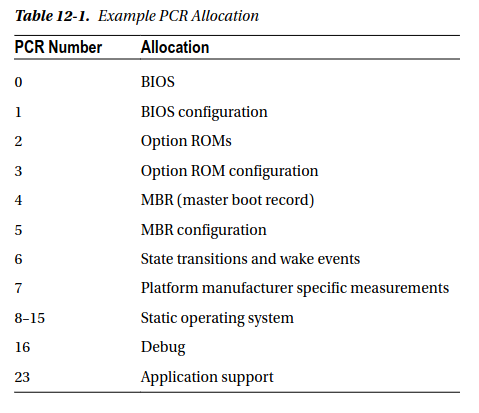
\includegraphics[width=0.8\textwidth]{figures/es-pcr.png} 
    \caption{Esempio di allocazione dei registri PCR.}\label{fig:allocazione_pcr}
\end{figure}

\subsection{Anonimizzazione delle chiavi (DAA)}\label{subsec:daa}
Da TPM 1.2 esiste anche il protocollo \textbf{DAA} (\textit{Direct Anonymous Attestation}), un meccanismo basato sul concetto di firme di gruppo. In questo schema, ogni entità coinvolta si fida e attesta reciprocamente l'autenticità delle altre, consentendo anche di dimostrare che una chiave è stata generata da un TPM senza rivelare né quale specifico TPM l'abbia creata, né informazioni a suo riguardo. 

La DAA rappresenta una forma di \textit{attestation} basata su metodi a \textit{zero knowledge} (\textit{direct proof}) e non necessita di una CA esterna, eliminando di fatto la necessità di un'entità terza esterna per la verifica. Questa funzionalità è particolarmente utile per stabilire se un sistema remoto con cui si sta comunicando è dotato di un TPM, senza esporre informazioni sensibili sull’identità del dispositivo.

La DAA sfrutta le chiavi AIK, descritte precedentemente. Il vantaggio di questo protocollo è che permette al creatore dell'AIK di scegliere una quantità variabile di informazioni che desidera trasmettere all’esterno, variando dall'anonimato perfetto (viene inviata la prova che un'AIK appartiene a un TPM, ma non quale) alla conoscenza perfetta (viene inviata la prova che una certa EK è associata a quella AIK). La differenza tra i due è evidente quando un TPM viene compromesso e la chiave privata di una particolare EK viene divulgata su Internet. A questo punto, una \textit{privacy CA} può revocare i certificati se sa che un certificato che ha creato è associato a quella particolare EK compromessa.

\subsection{Standardizzazione}
A partire dal TPM 1.2 il TCG decide di rendere la specifica TPM uno standard. Viene fornita un'interfaccia software standard e una configurazione dei pin del pacchetto più specifica rispetto alla 1.1b. Si mantiene comunque la compatibilità binaria del software per la versione 1.1b. 

\subsection{Attacchi a Dizionario}
Dopo il rilascio della 1.1b, il TCG si accorse immediatamente che il TPM non prevedeva alcuna resistenza agli attacchi a dizionario: non esistevano protezioni contro un aggressore che provava una password dopo l'altra nel tentativo di individuare quella corretta. La soluzione si individuò in maniera semplice, prevedendo un limite superiore ai tentativi di inserimento delle password per l’autorizzazione alla decifratura della chiave entro un certo intervallo temporale.

\subsection{NVRAM}
Durante lo sviluppo della specifica insorgono due punti problematici che richiedono un intervento progettuale:
\begin{enumerate}
    \item Il TPM è in grado di generare chiavi private, ma non dispone di memoria interna permanente per conservarle. Per ovviare a questa limitazione, può cifrare le chiavi con una chiave pubblica e archiviarle su disco, consentendo un recupero illimitato senza occupare spazio interno. Tuttavia, questo metodo diventa inapplicabile quando il sistema è spento, poiché, ad esempio, un disco crittografato non può contenere la propria chiave di decrittazione.
    \item Un'ulteriore criticità riguarda la gestione dei certificati di chiave di approvazione. Inizialmente, questi venivano memorizzati su disco, ma tale approccio si è rivelato inefficace, poiché le aziende spesso eseguivano una formattazione completa del sistema, eliminando involontariamente i certificati.
\end{enumerate}

Per questi motivi, ora il TPM contiene una piccola quantità di memoria ad accesso casuale non volatile, nota come \textbf{NVRAM} (\textit{Non-Volatile Random Access Memory}). Essa può essere utilizzata per memorizzare chiavi o dati, mantenerli al sicuro mentre la macchina è spenta, oppure come cache per le chiavi. Il software può anche utilizzare il TPM per creare contatori a incremento monotono protetti. Principalmente serve per mantenere al sicuro le \textit{Storage Root Keys} per le catene di certificati e la \textit{Endorsement Key}. 

Un \textit{NVRAM index} in un TPM è un'entità di memoria non volatile configurabile dall’utente per l’archiviazione di dati specifici. La NVRAM è lo spazio fisico disponibile nel TPM, mentre gli \textit{NV Index} rappresentano i blocchi logici configurabili all'interno di essa. Ogni \textit{NV Index} è identificato da un numero univoco e da un insieme di attributi personalizzabili che determinano il suo comportamento. 

A differenza degli oggetti standard del TPM, gli \textit{NV Index} dispongono di un numero maggiore di attributi, consentendo un controllo più granulare sulle operazioni di lettura e scrittura. Ogni indice è associato a una gerarchia al momento della creazione. Se la gerarchia viene cancellata, tutti gli \textit{NV Index} collegati vengono eliminati. Inoltre, dispongono di un valore di autorizzazione modificabile dal proprietario e di una policy di autorizzazione immutabile dopo la creazione.

\subsection{Timestamps}
Parlando di implementazioni di meccanismi di sicurezza tramite crittografia, non si può trascurare l'importance dei \textit{timestamps}. Questi risultano fondamentali sia per la generazione di numeri pseudo-casuali, sia per garantire l’univocità dei messaggi, determinare il tempo trascorso tra due tentativi di inserimento della chiave, verificare la scadenza di un certificato o di una firma digitale, e molte altre applicazioni crittografiche.

Il TPM trarrebbe grande vantaggio dalla presenza di un orologio interno indipendente dalla macchina ospitante. Tuttavia, il fatto stesso che il TPM sia un chip saldato alla scheda madre lo rende inevitabilmente dipendente dall’alimentazione della piattaforma. Una soluzione più pratica e meno onerosa fu l’idea di prevedere un modulo oscillatore che può sincronizzarsi con un orologio esterno, ma che è in grado di generare \textit{timestamp} firmati usando il proprio riferimento interno.

\clearpage
\section{La specifica 2.0}
Nel 2014 il TCG annuncia lo sviluppo di una nuova versione, che continua a ricevere aggiornamenti e modifiche anche negli ultimi anni. La specifica TPM 2.0 introduce numerose differenze nell’architettura del componente, principalmente dovute alla necessità di disaccoppiare la specifica da un singolo algoritmo (come SHA-1). In sostanza, il TPM 2.0 include nuovi algoritmi crittografici, nuove funzioni hash, lavora con chiavi più grandi ed è più flessibile nel gestire i suoi registri e la memoria sicura. Per ottenere queste modifiche, l’architettura è stata progettata da zero, così da ottenere un \textit{design} più pulito. 

Per ottenere quella maggiore flessibilità e per consentire un uso più diffuso della specifica, il TPM 2.0 viene stilato con un approccio "a libreria". Questo consente agli utenti di scegliere gli aspetti applicabili delle funzionalità del TPM con diversi livelli di implementazione e di sicurezza. Esiste però un dibattito sulla vera utilità della flessibilità: un’eccessiva libertà nello scegliere meccanismi potrebbe rappresentare un punto di caduta della sicurezza, un “assist” involontario ad un ipotetico attaccante. 

Dopo l’approccio a libreria, il TCG decise anche che la specifica doveva essere compilabile. Una specifica compilabile ha il vantaggio di ridurre notevolmente l'ambiguità: consiste in diversi documenti che descrivono il comportamento del codice, e questi sono derivati direttamente dal codice TPM 2.0, garantendo così un comportamento uniforme. Il codice di riferimento è ottenuto dall’implementazione autorevole di un emulatore, costruito direttamente dal TCG.

\subsection{Evoluzione da 1.2 a 2.0}
Il TPM 1.2 e le versioni precedenti erano limitati all'utilizzo dell'algoritmo RSA per la crittografia e dell'algoritmo SHA-1 per l'hashing crittografico. Nelle prossime sezioni verranno analizzate queste due problematiche.

\subsubsection{La debolezza di SHA-1}
Inizialmente il TCG scelse lo SHA-1 per la sua robustezza rispetto a MD5, che in quegli anni si stava rivelando vulnerabile. Lo SHA-1 però non resistette molto più a lungo: dal 2005 emersero attacchi crittografici che ne ridussero la resistenza alle collisioni. 

Il TCG, prevedendo l’inevitabile superamento di questo algoritmo, adottò diverse precauzioni: i comandi TPM concatenano ai dati valori freschi generati casualmente o sconosciuti dall’esterno del chip prima di eseguire le operazioni di hashing. Inoltre, l’utilizzo di strutture e formati fissi nei parametri dei comandi rende molto più difficile manipolare i dati ed ottenere un attacco di collisione efficace.

Con il tempo, la comunità crittografica ha iniziato a sostituire SHA-1 con algoritmi più sicuri come SHA-2. Il \textit{National Institute of Standards and Technology} (NIST) eliminò gradualmente lo SHA-1 a favore della famiglia SHA-2, per poi lavorare su un nuovo algoritmo, lo SHA-3. In risposta a questi cambiamenti, il TCG iniziò a lavorare sulla versione TPM 2.0, che non avrebbe codificato specificamente un algoritmo di \textit{digest}, ma avrebbe incluso un “identificatore di algoritmo”, permettendo di fatto una maggiore flessibilità senza dover modificare la specifica TPM ad-hoc.

Il TPM contiene una serie di comandi per un motore SHA-1 \textit{general purpose}. Questi comandi vengono esposti dal TPM per tutte quelle piattaforme che, al momento dell’invocazione, non dispongono di memoria sufficiente per eseguire operazioni SHA-1 in autonomia. È qui che si raggruppano tutti i possibili problemi dati dagli attacchi a collisione.

\subsubsection{La lentezza di RSA ed i suoi limiti}
Il TPM 1.2 e le versioni precedenti utilizzavano esclusivamente \textbf{RSA} (\textit{Rivest-Shamir-Adleman}) per la crittografia, un algoritmo asimmetrico che si presta a crittografare messaggi molto piccoli e veniva principalmente usato per scambiare chiavi di crittografia simmetrica. Non è adatto per crittografare grandi flussi di dati e richiede operazioni lente - motivo per cui la specifica 1.2 richiedeva che ogni cifratura RSA venisse eseguita tramite una sola operazione - per evitare rallentamenti dovuti a numerose operazioni di cifratura in serie. 
Sebbene l'uso di crittografia simmetrica (come \textbf{AES} [\textit{Advanced Encryption Standard}] o \textbf{DES} [\textit{Data Encryption Standard}]) avrebbe semplificato notevolmente la specifica del TPM, c’erano dei requisiti legali stringenti per l'esportazione di chip crittografici simmetrici dagli Stati Uniti, quindi si optò per RSA. Limitare il TPM a crittografare dati e chiavi con RSA implicò la realizzazione di alcune scorciatoie di \textit{design} non banali.

RSA rimane comunque un algoritmo poco efficiente, e nel tempo la dimensione della chiave che veniva usata dal TPM diventava sempre meno sicura. Il TPM 1.1b aveva strutture attentamente progettate in modo che le strutture tradotte in flussi di byte fossero abbastanza compatte da essere crittografate con una chiave RSA da 2.048 bit in una sola crittografia. Ciò significava che c'erano solo 2.048 bit (256 byte) con cui lavorare.

Per adottare una flessibilità in termini di algoritmi, diventa necessario poter fornire \textit{digest} potenzialmente più grandi dei 20 byte di SHA-1: era chiaro che le strutture esistenti erano troppo piccole. Una chiave RSA non poteva crittografare le strutture in serie tramite una sola operazione e allo stesso tempo utilizzare più operazioni per crittografare le strutture in blocchi era impraticabile. Aumentare la dimensione della chiave RSA avrebbe significato utilizzare dimensioni di chiave che non erano ampiamente usate nell'industria e avrebbe anche aumentato i costi, cambiato le strutture delle chiavi e rallentato il chip.

Tutti questi temi hanno portato alla necessità di un'evoluzione, che si è concretizzata nel passaggio alla versione successiva. Prima dello sviluppo di TPM 2.0 vengono abrogate le leggi che imponevano limiti al commercio di dispositivi per la crittografia simmetrica. Anche per questo il TCG decise che la specifica doveva utilizzare la pratica comune di crittografare una chiave simmetrica con la chiave asimmetrica e i dati con la chiave simmetrica. Le operazioni con chiave simmetrica sono ben adatte per crittografare grandi flussi di byte, perché sono molto più veloci delle operazioni asimmetriche. 
La crittografia con chiave simmetrica ha quindi rimosso il limite sulla dimensione delle strutture da cifrare, in quanto l’esecuzione di un elevato numero di operazioni crittografiche simmetriche in sequenza non comporta significativi rallentamenti prestazionali, anche in presenza di grandi volumi di dati.

\subsection{I casi d’uso 2.0}
Oltre a risolvere le problematiche legate all’utilizzo puro della crittografia RSA e alla funzione di hash SHA-1, il TPM 2.0 aggiunge nuove funzionalità e caratteristiche, come l'agilità degli algoritmi e la capacità di implementare nuovi algoritmi crittografici secondo necessità.

Negli anni, il gruppo TCG selezionò le caratteristiche principali del progetto e si stabilì su un set di funzionalità di base e un \textit{design} di alto livello: venne deciso di cambiare tutte le strutture per consentire l'indipendenza dagli algoritmi, un concetto detto "\textit{Algorithm Agility}". 

Tutte le tecniche di autenticazione furono unificate in una sola tecnica, la "\textbf{EA} (\textit{Enhanced Authorization})". Questo accentramento del controllo aumentò la flessibilità dei meccanismi di autorizzazione, riducendo contemporaneamente i costi di implementazione e la difficoltà cognitiva di comprendere la specifica. 

Questi due punti sono forse i più salienti e rivoluzionari rispetto alla specifica precedente. Tuttavia non sono gli unici e di seguito è possibile trovare una descrizione per le principali funzionalità intese come casi d’uso.

\subsubsection{Algorithm Agility}
Nell’introduzione della sezione dedicata ai casi d’uso viene anticipato che TPM 1.2 faceva uso di un “trucco di progettazione” per poter risparmiare tempo, risorse e spazio durante la cifratura delle chiavi solo RSA.
L’\textit{escamotage} sfrutta la base matematica delle chiavi di RSA: una chiave privata RSA è composta da due numeri primi molto grandi, elaborati in qualche modo, e la chiave pubblica è il loro prodotto. Con la chiave madre veniva cifrato solo uno dei due numeri necessari per la coppia di chiavi. La conoscenza di uno solo dei due non porta vantaggi all’attaccante (in caso la chiave abbia una dimensione ragionevole e dunque quest’ultimo non possa “indovinarla”). Questo processo permetteva di ridurre la quantità di dati che dovevano essere crittografati ed eliminava la necessità che il TPM contenesse un algoritmo simmetrico. 

Tuttavia questo meccanismo artificioso è lento. 

Unendo questo fatto con altri due punti:
\begin{enumerate}
    \item dopo il rilascio della 1.2, gli Stati Uniti rimuovono alcuni vincoli legali sull’\textit{export} delle tecnologie che montano implementazioni di crittografia simmetrica;
    \item un coprocessore crittografico idealmente conosce sia algoritmi simmetrici che asimmetrici.
\end{enumerate}
Il TCG raggiunge la conclusione di progettare la nuova specifica in modo da permettere l’implementazione di entrambi i tipi di algoritmi.

Nel TPM 2.0, le chiavi \textit{general purpose} usate durante le operazioni TPM sono generalmente memorizzate crittografate simmetricamente, fuori dal chip. La chiave simmetrica che cifra la chiave memorizzata all’esterno è a sua volta cifrata, da una chiave detta \textbf{KEK} (\textit{Key Encryption Key}). Questo processo a due fasi aggiunge pochissimo sovraccarico di tempo di esecuzione rispetto al metodo artificioso sviluppato per TPM 1.2.

A questo punto però il TPM non è ancora “pronto” all’implementazione di nuovi algoritmi: le strutture delle chiavi rispecchiano perfettamente ancora le dimensioni degli hash SHA-1. Soffermandosi sulla funzione di hash, non era possibile sostituire semplicemente l'algoritmo SHA-1 con SHA-256 (l’algoritmo successore di SHA-1). I 12 byte aggiuntivi in SHA-256 rendevano la struttura dei dati risultante troppo grande per essere crittografata in un solo passaggio con una chiave RSA.

Possiamo concludere che preparare la specifica all’utilizzo di crittografia non-strettamente RSA è la naturale evoluzione del TPM 1.2. Il TCG decise di cambiare completamente la struttura delle chiavi, per svincolarsi dalla coppia RSA -- SHA-1.
Questo cambiamento permette di utilizzare qualsiasi combinazione di algoritmi nella specifica indipendentemente dalle dimensioni delle chiavi. Gli algoritmi supportati vengono codificati in una tabella di \textbf{ID} (\textit{Identifier}) algoritmi indipendente dalla specifica stessa. 

Nel TPM 2.0 la tabella degli \textbf{ID} algoritmi elenca algoritmi di crittografia, algoritmi di hash, funzioni di derivazione delle chiavi (\textbf{KDF} [\textit{Key Derivation Function}]), schemi di firma e altre informazioni essenziali alla corretta esecuzione delle funzionalità di sicurezza del TPM. La tabella può essere inserita in un’implementazione assegnando semplicemente un numero per rappresentare l’aggiunta di un algoritmo. Il TCG comunque fornisce set obbligatori di algoritmi associati ai vari TPM fisici, in funzione della piattaforma su cui la specifica verrà implementata. Questo dettaglio garantirà un'interoperabilità di base tra le varie implementazioni! 

\subsubsection{Enhanced Authority}
Nel TPM 2.0 vengono ripensate anche le gerarchie di chiavi. Rimane il concetto di \textit{Endorsement Key} per firma o attestazione e la SRK per la crittografia dei dati. Queste due categorie sono associate a due semi, “\textit{Endorsement seed}” e “\textit{Storage seed}”:
Il primo genera chiavi usando un \textit{template} noto e rigido, saranno chiamate EK. Queste chiavi figlie servono principalmente per le \textit{policies} (o meglio, a rappresentare l’autorizzazione all’utilizzo di una certa \textit{policy} di sicurezza) e corrispondono a “sessioni” di utilizzo dei comandi TPM.
Il secondo genera chiavi che non sono usate per attestazioni, ma chiavi che serviranno come “madri” per un’altra catena di chiavi usata per cifrare dati.

La necessità di avere una categoria di chiavi che danno origine a catene di chiavi sempre più sicure ed importanti, nasce da un dato pratico: nel TPM 1.2 la chiave SRK era nota (20 byte impostati a zero -- in gergo \textit{well known secrets}) e questo portava ad un abuso della \textit{Owner Authorization}. 

\begin{figure}[htbp]
    \centering
    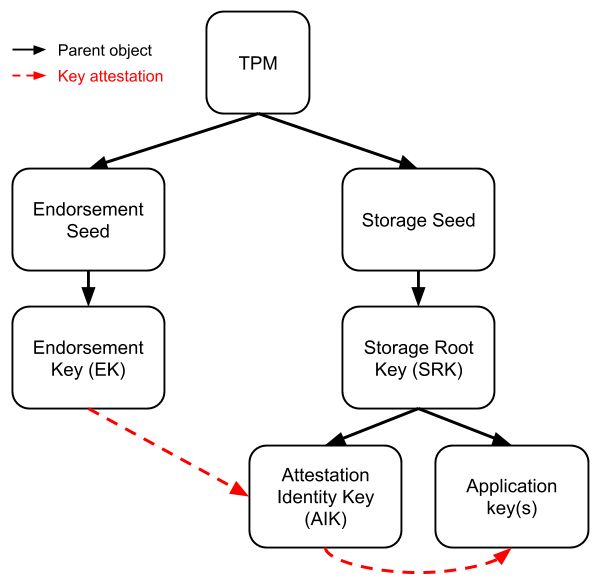
\includegraphics[width=0.55\textwidth]{figures/gerarchia-seed.png}
    \caption{Gerarchie dai seed TPM.}
    \label{fig:gerarchie_seed_tpm}
\end{figure}

In TPM 1.2, l'autorizzazione (il processo mediante il quale il software dimostra al TPM di essere autorizzato a utilizzare un oggetto) funziona tramite accesso con password e valori PCR. Per utilizzare una chiave, il software dovrà dimostrare la conoscenza dell'hash della password come parte del comando. L’\textit{Owner} era l’entità che conosceva la password, ma non era previsto distinguere tra un \textit{admin}, un utente o un manutentore per esempio. Quando più utenti condividono una piattaforma, diventa difficile condividere chiavi e dati TPM. Avere lo stesso meccanismo di autenticazione rende difficile gestire tanti ruoli in maniera indipendente ed efficace.

Dal TPM 2.0 i ruoli diventano concetti separati e previsti esplicitamente dalla specifica: esistono diverse autorizzazioni e \textit{policies} da combinare assieme, le responsabilità vengono distribuite su più gerarchie. Oltre alle due già citate (corrispondenti a \textit{endorsement seed} e \textit{storage seed}) la nuova specifica 2.0 prevede due gerarchie aggiuntive:
\begin{itemize}
    \item \textbf{Endorsement Hierarchy, \textbf{EH} (\textit{Endorsement Hierarchy}).} Utilizzata per tutte le operazioni sensibili alla privacy, autenticazione e per l'attestazione del dispositivo. Serve per generare certificati di identità e la chiave principale è la EK. Ogni dispositivo TPM ha un'unica EK che viene utilizzata per generare chiavi subordinate (AIK) per scopi di attestazione.
    \item \textbf{Storage Hierarchy, \textbf{SH} (\textit{Storage Hierarchy}).} Destinata all'uso del proprietario della piattaforma (azienda o l'utente finale). Utilizzata per operazioni non legate alla privacy, come la crittografia per proteggere i dati e la gestione delle chiavi di sessione. Praticamente replica la famiglia SRK della specifica precedente.
    \item \textbf{Platform Hierarchy, \textbf{PH} (\textit{Platform Hierarchy}).} Gerarchia definita dal produttore del chip, viene utilizzata per le funzioni di manutenzione e amministrazione. Le chiavi in questa gerarchia sono usate dagli aggiornamenti \textit{firmware}, \textbf{BIOS} (\textit{Basic Input/Output System}) etc. Non riguarda l’utente finale.
    \item \textbf{Null Hierarchy, \textbf{NH} (\textit{Null Hierarchy}).} Possiede il suo \textit{seed} unico, con chiavi primarie e derivate che però non possono essere preventive e persistenti. Il \textit{seed} è rigenerato a ogni reset del TPM: queste chiavi sono sempre effimere. 
\end{itemize}

L'Enhanced Authorization espande notevolmente i metodi con cui l'uso di chiavi e dati può essere autorizzato. In TPM 1.2, prima di ogni comando TPM ne veniva inviato un altro, che richiedeva l'autorizzazione per avviare la sessione: uno dei parametri del comando era un codice di autenticazione del messaggio, un hash della password che proteggeva l’accesso al comando stesso.

La EA estende queste sessioni di autorizzazione in \textit{policy sessions}, che permettono di combinare più metodi di autorizzazione (o politiche di autorizzazione) tramite logica booleana, creando di fatto un linguaggio di politica flessibile.  

Dal punto di vista operativo, la politica di sessione viene creata a livello software e poi associata ad un hash. Quando un comando TPM necessita di una certa politica, diventa sufficiente specificare l’hash ed il TPM avvierà una sessione di autorizzazione e invierà un comando dedicato per ogni \textit{token} di autorizzazione. Il TPM verificherà se l’hash della sequenza di comandi (con relativi input) sia lo stesso dell'hash della politica specificato al momento della creazione.

Per completezza, si sottolinea che non solo viene elaborato il nuovo meccanismo di politiche di autorizzazione, ma si prevedono nuovi metodi di autenticazione. Alcuni di questi sono: chiave HMAC del software, firma digitale, firma con dati aggiuntivi (forniti ad esempio da un lettore biometrico di impronte), indice della NVRAM o località di origine del comando.

\subsubsection{Quick key loading}
Nel TPM 1.2, la prima volta che una chiave veniva caricata, era necessario un processo di decodifica della chiave privata mediante l'uso della chiave privata del genitore della chiave stessa. Tale operazione risultava relativamente lenta. Per evitare la necessità di ripetere questa decodifica più volte durante una sessione, il TPM memorizzava temporaneamente la chiave decodificata nella sua \textit{cache}. Poiché si trattava di chiavi composte da una parte pubblica e una privata, l'esposizione della chiave pubblica non comportava rischi di compromissione. Sebbene il processo non utilizzasse crittografia simmetrica, questa soluzione consentiva al TPM di mantenere la chiave "pronta all'uso" durante l'intero ciclo di alimentazione, garantendo un accesso più rapido alla chiave nelle operazioni successive.

Durante il singolo ciclo di alimentazione, il TPM poteva ricaricare la chiave più velocemente rispetto alla ripetuta decodifica con la chiave privata del genitore. Tuttavia, al termine della sessione, e quindi con lo spegnimento, la chiave veniva cancellata e alla successiva accensione era necessario ripetere il processo di decodifica.

Con TPM 2.0, invece, a meno che una chiave non venga importata dall'esterno nel TPM, le chiavi memorizzate utilizzando memoria esterna sono cifrate con una chiave simmetrica. Questo approccio consente un caricamento rapido delle chiavi, eliminando la necessità di utilizzare una \textit{cache} per spostarle, a meno che non sia necessario l'accesso a una chiave genitore. Poiché il processo di decodifica è tanto veloce quanto il recupero di una chiave dalla \textit{cache}, non c'è motivo di usarla. Questo miglioramento permette un caricamento delle chiavi più efficiente, consentendo a più utenti di utilizzare un TPM senza riscontrare ritardi significativi. Di conseguenza, diventa più semplice progettare sistemi in cui più applicazioni possano accedere a un TPM in modo apparentemente illimitato.

\subsubsection{Non-brittle PCRs}
Nei primi modelli di TPM, in particolare nella versione 1.0, una delle principali problematiche era la fragilità dei valori PCR. I PCR registrano lo stato della macchina in diversi momenti del processo di avvio: i numeri più bassi rappresentano le prime fasi del \textit{boot}, mentre quelli più alti riflettono eventi successivi, fino all'avvio del sistema operativo. Per garantire maggior sicurezza, è possibile vincolare l'accesso a determinate chiavi e dati a specifici valori PCR, un meccanismo noto come \textit{sealing}. Tuttavia, questo approccio presentava alcune criticità, in particolare durante gli aggiornamenti del BIOS: se un segreto era bloccato a un valore PCR dipendente dal BIOS, un aggiornamento lo avrebbe reso inaccessibile, costringendo a sbloccarlo prima dell'operazione e a riassociarlo successivamente.

La specifica TPM 2.0 introduce un sistema più flessibile che consente di vincolare l’accesso alle risorse non a un valore PCR fisso, ma a una firma digitale rilasciata da un’entità di fiducia. Questo permette di recuperare i dati in più configurazioni approvate, ad esempio in base a versioni del BIOS validate da un'organizzazione IT o dal produttore dell’hardware. In questo modo, le risorse non sono più bloccate rigidamente a un singolo stato del sistema, ma possono essere recuperate in più configurazioni approvate.

I PCR permettono di bloccare alcuni valori tramite “\textit{sealing}”. Ma se questi valori sono chiavi o dati che rappresentano il BIOS, potrebbero presentarsi problemi qualora un valore serva prima dell’avvio del BIOS, prima fra tutte la casistica di \textit{update} al BIOS! Questa complicazione si chiama fragilità del PCR (o \textit{brittle PCR}). Questa maggiore flessibilità è resa possibile dal comando \texttt{TPM2\_PolicyAuthorize}, che permette di definire criteri di accesso dinamici (sulla base di EA). 

\subsubsection{Flexible Management}
La specifica 1.0 prevedeva due soli tipi di autorizzazione: quella della SRK e la \textit{owner authorization}. Spesso la SRK era settata a 20 bit tutti nulli ed utilizzata per molteplici scopi, rendendo difficile la gestione indipendente di tanti ruoli. La famiglia TPM 1.2 permetteva la delega, ma era complicata e raramente usata.

In TPM 2.0 vengono analizzati i diversi casi in cui l’autorizzazione tramite SRK veniva utilizzata e da questi sono ricavati diverse gerarchie di chiavi. Le gerarchie sono pensate per occuparsi di autorizzazioni e \textit{policy} diverse, rendendo la gestione di chiavi (e utenti) più leggera. Una descrizione più dettagliata delle gerarchie è stata fornita nella sezione 3.5.1.2.1 Le gerarchie.

\subsubsection{Identifying resources}
Nella specifica TPM 1.2, le risorse venivano identificate tramite un \textit{handle} anziché un nome legato alla risorsa stessa. Questo approccio apriva alla possibilità che un software di basso livello potesse modificare l'\textit{handle} identificativo, rendendo possibile indurre l’utente ad autorizzare un'azione diversa da quella che pensava di approvare. In tal modo, si creava una vulnerabilità che permetteva la manipolazione delle autorizzazioni.

Con l'introduzione del TPM 2.0, le risorse vengono ora identificate tramite un nome, che è vincolato alla risorsa, eliminando di fatto la vulnerabilità descritta. Inoltre, diventa possibile utilizzare una chiave TPM per firmare questo nome, garantendo così la sua correttezza. Il nome viene composto in modo da comprendere la \textit{policy} di autorizzazione della chiave, quindi firmare il nome equivale a firmare e validare le modalità attraverso cui è possibile autorizzare l'uso di una chiave. Questa firma funge anche da prova dell'integrità e dell'affidabilità della chiave, come descritto nel capitolo sull’EA. Se la chiave viene duplicata, la firma può fornire un "certificato di nascita", dimostrando quale TPM è stato utilizzato per la sua creazione.

\section{Variazioni del TPM 2.0}
Dalla specifica 2.0, il TPM diventa sempre più facile da implementare su diverse piattaforme, da PC a server a \textbf{SoC} (\textit{System on Chip}). Esistono quattro tipi principali di “forma di TPM” al momento, ognuna con i suoi pro e contro. In base al livello di sicurezza richiesto da un ambito è doveroso fare una valutazione dei costi e dei rischi per selezionare la forma che meglio si presta all’utilizzo specifico.

\subsection{Discrete TPM}
La forma del \textit{discrete} TPM (dTPM) è pensata per gli ambiti di sicurezza più alta e mira a rendere il dispositivo inviolabile, anche contro attacchi sofisticati. Per garantire questa protezione, il chip viene progettato e testato secondo standard rigorosi, resistendo a manomissioni avanzate come il \textit{probing} o il congelamento.

Si tratta di un modulo hardware fisicamente isolato e autonomo, integrato come un chip dedicato e collegato alla \textbf{CPU} (\textit{Central Processing Unit}) tramite un'interfaccia sicura. Le interfacce più comuni sono LPC (Low Pin Count), \textbf{I2C} (\textit{Inter-Integrated Circuit}), \textbf{SPI} (\textit{Serial Peripheral Interface}) e, occasionalmente, \textbf{PCIe} (\textit{Peripheral Component Interconnect Express}). L’uso di un collegamento dedicato riduce i rischi legati a interfacce condivise, limitando l’esposizione ad attacchi di intercettazione del \textit{bus} di comunicazione.

Il dTPM è adatto a proteggere sistemi critici, come nel controllo dei freni di un'automobile o di valvole in impianti che trattano materiali pericolosi. 

\subsection{Integrated TPM}
L'Integrated TPM (iTPM) rappresenta un livello di sicurezza inferiore rispetto al TPM discreto. Pur essendo una soluzione hardware, è integrato in un chip che svolge anche altre funzioni (come la CPU o il chipset). Risulta meno resistente alle manomissioni perché non possiede un’area isolata. Tuttavia, grazie alla sua implementazione hardware, mantiene una certa protezione contro le vulnerabilità \textit{software}. Questa soluzione offre un compromesso tra costi, prestazioni e sicurezza, perché mantiene comunque un buon livello di risorse di sicurezza dedicate.

\subsection{Firmware TPM}
Il \textit{firmware} TPM (fTPM) è una soluzione implementata tramite \textit{software} protetto, eseguibile direttamente sulla CPU principale senza la necessità di un chip separato. Il codice opera all'interno di un ambiente di esecuzione protetto, noto come \textbf{TEE} (\textit{Trusted Execution Environment}), che lo isola dagli altri programmi in esecuzione sulla CPU. In questo modo, informazioni sensibili come chiavi private, possono essere conservate nel TEE, rendendo più complesso l’accesso per eventuali attaccanti.

A differenza di un TPM hardware, l'fTPM non offre resistenza fisica alle manomissioni e la sua sicurezza dipende da diversi fattori, tra cui il sistema operativo del TEE e la presenza di vulnerabilità nel codice delle applicazioni eseguite al suo interno. Gli fTPM sfruttano il processore del sistema ospitante per creare un perimetro logico sicuro, basandosi su tecnologie hardware come \textbf{ARM} (\textit{Advanced RISC Machine}) TrustZone, Intel \textbf{SGX} (\textit{Software Guard Extensions}) e Intel Management Engine.

Dunque gli fTPM dipendono fortemente dalla capacità della CPU della piattaforma \textit{host} nel fornire un ambiente sicuro. Tuttavia se l’implementazione viene realizzata e progettata con le dovute accortezze, può garantire un buon livello di sicurezza.

\subsection{Software TPM}
Il \textit{Software} TPM (sTPM) è una soluzione implementata come un emulatore \textit{software} del TPM. Tuttavia, questa tipologia di TPM presenta numerose vulnerabilità, sia come possibilità di manomissione sia a causa della forte dipendenza da eventuali \textit{bug} nel sistema operativo su cui viene eseguita.

Gli sTPM non offrono protezione contro attacchi fisici o informatici e non sono considerati affidabili per applicazioni che richiedono un elevato livello di sicurezza. Un aspetto interessante è il loro utilizzo anche in ambienti \textit{cloud}, dove vengono implementati a livello di \textit{hypervisor} per la gestione della sicurezza virtualizzata.

Nonostante le sue limitazioni in termini di sicurezza, l’sTPM ha applicazioni specifiche, risultando particolarmente utile per attività di test o per la progettazione di prototipi di sistemi che prevedono l’integrazione di un TPM senza la possibilità di operare direttamente su un chip. In questi contesti, può rappresentare una soluzione adeguata per la sperimentazione e la validazione del \textit{software}.

\subsection{Virtual TPM}
Molti sistemi \textbf{IoT} (\textit{Internet of Things}) includono sensori e elaborazione \textit{cloud}, il che implica l’impiego di tecniche di virtualizzazione. L'uso delle macchine virtuali (\textbf{VM} [\textit{Virtual Machine}]) sicuramente offre flessibilità nell'elaborazione dei dati, ma aumenta sensibilmente anche il rischio di attacchi a causa della sua natura virtuale.

L'integrazione di un Virtual TPM (vTPM) consente di verificare l'assenza di attività malevole prima dell'avvio del processo di \textit{boot} di una macchina virtuale, rafforzando così la sicurezza del sistema. 

In un ambiente \textit{cloud}, il vTPM si inserisce come una soluzione intelligente per la protezione, in quanto fa parte dell'infrastruttura basata su \textit{cloud} e distribuisce i comandi a ciascuna macchina virtuale separatamente. A differenza di un TPM tradizionale, che si concentra sulla protezione del dispositivo \textit{host}, il vTPM è progettato per proteggere gli ambienti virtualizzati, dove più macchine virtuali, ognuna con il proprio sistema operativo, possono essere eseguite su un singolo \textit{host}. 

Il vTPM emula le funzionalità di archiviazione sicura di un TPM hardware e compie operazioni crittografiche direttamente nel \textit{software}, offrendo gli stessi comandi di un TPM fisico. Consente al sistema operativo \textit{guest} di generare e conservare chiavi private, migliorando così le misure di sicurezza disponibili. Le chiavi vengono isolate dal sistema principale, riducendo il rischio di compromissione durante eventuali attacchi. Il vTPM riceve informazioni crittografiche da un'autorità di certificazione (CA), simile alla chiave di crittografia (EK) di un TPM fisico, e le chiavi generate vengono utilizzate esclusivamente dal sistema operativo per operazioni di crittografia e firma digitale. Ciò consente la validazione remota dell'identità e dell'affidabilità della macchina virtuale, così come la verifica del \textit{software} in esecuzione.

Tuttavia, nonostante i vantaggi, i vTPM presentano alcune vulnerabilità. Poiché sono implementati tramite \textit{software}, sono soggetti ad attacchi legati alle debolezze del sistema operativo sottostante e della virtualizzazione stessa. L'isolamento offerto dal vTPM dipende fortemente dalla sicurezza dell'infrastruttura di virtualizzazione. Inoltre, i vTPM non offrono la stessa resistenza fisica alle manomissioni dei TPM hardware, il che li rende più suscettibili ad attacchi mirati.
\chapter{\acrshort{tpm} Software Stack}\label{ch:tss}

Il \acrshort{tcg} definisce un'interfaccia software per il \acrshort{tpm}v1.2, chiamata \acrlong{tss} (\acrshort{tss}), con lo scopo di fornire un'interfaccia verso il \acrshort{tpm} che permetta a quanti più programmatori un facile e immediato utilizzo, ma anche un'interfaccia che ponesse una base comune per tutte le piattaforme e per tutti i \acrshort{tpm}. Il \acrshort{tss} è quindi un'\acrshort{api} standard per accedere alle funzioni del \acrshort{tpm}, pensato per incentivare la diffusione di applicazioni adatte ad un \textit{computing} più resistente alla manomissione. Il \acrshort{tss} mira anche a fornire mezzi affinché le applicazioni possano comunicare con i \acrshort{tpm}, sia localmente che da remoto - una sfida non banale, se si pensa alla natura non sicura delle reti Internet.

Il \acrshort{tcg} lavora con l'obiettivo di produrre una specifica neutrale rispetto ai produttori hardware in modo che i venditori di applicazioni possano scrivere applicazioni che funzioneranno indipendentemente dalla piattaforma, dal sistema operativo o dall'ambiente utilizzato. 

Operativamente il \acrshort{tss} agisce da libreria, offrendo un'interfaccia di programmazione semplificata rispetto a quelli che altrimenti sarebbero dei comandi molto complicati e strutturati. Il \acrshort{tss} converte le chiamate ad alto livello applicativo in comandi equivalenti per il \acrshort{tpm}, li invia al driver del dispositivo, che poi li trasmette fisicamente al chip.

I livelli della libreria sono: Feature \acrshort{api} (FAPI), Enhanced System API (ESAPI), System API (SAPI), \acrshort{tpm} Command Transmission Interface (TCTI), \acrshort{tpm} Access Broker (TAB), Resource Manager (RM) e Device Driver (DD).

Il Device Driver potrebbe avere un nome fuorviante: non è da intendere come i driver utilizzati dai \acrshort{so} per interfacciarsi con l'hardware. Anzi, questo è il componente che gestisce la trasmissione fisica dei dati.

\begin{figure}[htbp]
    \centering
        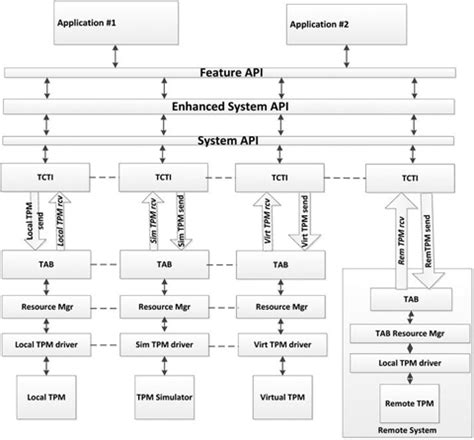
\includegraphics[width=0.7\textwidth]{figures/diagramma-tss.png}
    \caption{Diagramma del \acrshort{tss}, con un esempio per \acrshort{tpm} locale, un simulatore, un \acrshort{tpm} virtuale ed uno remoto.}
    \label{fig:diagramma_tss}
\end{figure}

\section{FAPI -- Feature API}\label{sec:fapi}

Il livello Feature \acrshort{api} (\acrshort{fapi}) nello stack software \acrshort{tpm} fornisce un set di \acrshort{api} di alto livello progettate per semplificare l'interazione con le funzionalità del \acrshort{tpm}. Questo livello offre un'interfaccia \textit{user-friendly} per sviluppatori, permettendo loro di accedere facilmente alle funzionalità di sicurezza avanzate del \acrshort{tpm} senza dover gestire la complessità delle \acrshort{api} di basso livello.

Su questo livello si scrivono la maggior parte delle applicazioni utente: è pensato proprio per essere il punto in cui i programmatori accedono alle funzionalità più comunemente utilizzate del \acrshort{tpm}. E' costruito pensando che la maggior parte dei programmi che usano il \acrshort{tpm}, non abbiano bisogno delle \acrshort{api} più profonde.

Il \acrshort{fapi} cerca anche di minimizzare il numero di chiamate che un'applicazione deve fare per ottenere qualcosa, ed il numero di parametri che deve definire. Per questo un'implementazione potrebbe prevedere file di impostazione, che definiscono selezioni \textit{default} di algoritmi, dimensioni delle chiavi, modalità ecc. Un meccanismo comodo per gli utenti finali che non dovrebbero più preoccuparsi di definire i dettagli di utilizzo del \acrshort{tpm} ad ogni chiamata.

Tutti gli oggetti creati e utilizzati dai comandi a livello \acrshort{fapi} devono essere autorizzati da una \textit{policy}, identificata dalla tag \texttt{TSS2\_POLICY\_AUTHVALUE}. I comandi per le \textit{policy} possono richiedere input esterno o no. Per il successo di questi comandi è necessario che il chiamante fornisca i parametri necessari -- tra i parametri ci sono proprio i valori su cui calcolare la correttezza della \textit{policy} -- perché il \acrshort{fapi} non è in grado di recuperare informazioni esterne.

Qui entra in gioco un meccanismo di \textit{callbacks}: le \textit{callback} sono registrate nel programma che parla con il \acrshort{fapi} cosicché questo possa sapere se serve una password, una selezione tra opzioni, o una firma. Ad esempio, per ottenere la password, la \textit{callback} è relativamente semplice, diventa sufficiente sfruttare una funzione - definita dall'applicazione che chiama l'\acrshort{api} -- per gestire l'interazione utente e recuperare l'input. 

Per quei comandi che non richiedono input esterno invece, le \textit{policy} fanno affidamento a dei \textit{check} sui valori nei \acrshort{pcr}, sulla \textit{locality} del comando, il \textit{counter} interno del \acrshort{tpm}, il codice che identifica il comando che richiede la verifica della \textit{policy}, l'hash del nome dell'oggetto inviato al \acrshort{tpm} ecc. Tutte queste modalità prevedono che sia il \acrshort{fapi} ad occuparsi della verifica richiesta.

Da notare che solitamente, una piattaforma possiede un solo \acrshort{tpm} che viene messo a disposizione di più applicazioni, con accesso mutualmente esclusivo. In realtà non è tassativo, e da una singola macchina si potrebbero usare \acrshort{tpm} simulati, remoti o fisici senza alcun limite.

\section{\acrshort{esapi} - Enhanced System \acrshort{api}}\label{sec:esapi}

Il livello Enhanced System \acrshort{api} (\acrshort{esapi}) fornisce \acrshort{api} di medio livello che offrono un maggiore controllo e funzionalità rispetto alle \acrshort{api} di basso livello (\acrshort{sapi}). 

Permette di gestire le sessioni in minima parte e supporta alcune delle capacità crittografiche rese disponibili dal \acrshort{tpm}. 

Questo livello è progettato e pensato per sviluppatori che necessitano di operazioni più dettagliate e personalizzate sulle funzionalità del \acrshort{tpm}, pur mantenendo un'interfaccia abbastanza semplice e senza necessitare di uno studio approfondito della specifica.

Il livello \acrshort{esapi} rappresenta le risorse che utilizza come una \textit{linked list}: ogni nodo consiste in una struttura contenente un \textit{handle} (un identificatore univoco per il nodo), la risorsa da memorizzare e un puntatore all'elemento successivo. 

\section{\acrshort{sapi} -- System \acrshort{api}}\label{sec:sapi}

Il livello System \acrshort{api} (\acrshort{sapi}) rappresenta un'\acrshort{api} di basso livello con accesso diretto e dettagliato alle funzioni del \acrshort{tpm}. È progettato per sviluppatori che necessitano del massimo controllo sulle operazioni del \acrshort{tpm}, permettendo loro di interagire direttamente con le primitive di sicurezza e gestire le risorse del \acrshort{tpm}. Viene richiamata ed utilizzata ogni volta che sono effettuate chiamate a basso livello come firmware, BIOS, applicazioni, sistemi operativi, ecc. 

Il \acrshort{sapi} è concettualmente ma anche concretamente uno spartiacque: i livelli sopra il \acrshort{sapi} esistono generalmente con corrispondenza uno ad uno per ogni processo che fa utilizzo del \acrshort{tpm}. I livelli al di sotto, sono solitamente specifici per piattaforma che dispone di \acrshort{tpm}.

La specifica del \acrshort{sapi} è pensata per essere utilizzabile su diverse piattaforme. Da sottolineare lo sforzo progettuale per permettere di minimizzare l'utilizzo della memoria: le implementazioni del \acrshort{sapi} possono evitare di allocare memoria, delegando la responsabilità al programma chiamante.

I comandi disponibili nel \acrshort{sapi} si dividono in quattro gruppi: \textit{context allocation functions}, \textit{preparation functions}, \textit{execution functions} e \textit{completion functions}. Di seguito una breve panoramica:

\begin{description}
    \item[\textit{context allocation functions}:] comandi che si occupano di allocare la struttura dati di \textit{context} necessaria per un comando \acrshort{sapi}. La struttura è definita dalle singole implementazioni e indica come vengono memorizzati i dati dello stato \acrshort{tpm} necessari per la corretta esecuzione di un comando.
    
    \item[\textit{preparation functions}:] alcune funzionalità del \acrshort{tpm} possono necessitare dello svolgimento di \textit{pre-processing} e \textit{post-processing}. Il meccanismo di ``preparazione'' dei parametri di un comando è chiamato \textit{marshalling}, e le \textit{preparation functions} hanno proprio questo ruolo: predispongono i parametri, ordinano flussi di byte, strutturano i dati, preparano le sessioni. Sono fondamentali per iniziare e concludere alcune chiamate di comandi \acrshort{tpm}.
    
    \item[\textit{execution functions}:] sono quei comandi che effettuano l'invio del comando e ne riceve le risposte - l'invio può essere sincrono o asincrono. Ci sono due modi per inviare comandi in modo sincrono: la prima prevede una sequenza di chiamate di funzione domanda-risposta (\textit{multi-chiamata}); la seconda è una chiamata unica. La necessità di supportare la modalità asincrona rispetto a quella sincrona e per la chiamata unica rispetto a un approccio \textit{multi-chiamata} non nasce da un motivo di progettazione, ma dall'idea di implementare il \acrshort{tss} per il maggior numero possibile di architetture applicative.
    
    \item[\textit{completion functions}:] gruppo di funzioni atte ad abilitare il \textit{post-processing} di un altro comando qualora necessario: ad esempio quando viene richiesto un calcolo \acrshort{hmac}, o una decifratura con verifica di integrità. Queste funzioni usano i parametri puntatore e dimensione del parametro di risposta, per prelevare i dati che vanno post-processati ed eseguire verifiche, calcoli o controlli che richiesti.
\end{description}

\section{\acrshort{tcti} -- \acrshort{tpm} Command Transmission Interface}\label{sec:tcti}

L'interfaccia \acrshort{tpm} Command Transmission Interface (\acrshort{tcti}) rappresenta un componente fondamentale del \acrshort{tss}, di fatto perché gestisce la trasmissione e la ricezione dei comandi tra l'applicazione.

La \acrshort{tcti} funge da ponte per l'invio di flussi di byte (un comando \acrshort{tpm} è un flusso di byte) dal \acrshort{tpm} alle applicazioni e viceversa. Fornisce un'interfaccia standardizzata che consente alle applicazioni di interagire con il \acrshort{tpm} senza che queste debbano gestire i dettagli specifici della comunicazione con il dispositivo, semplificando anche l'uso dei comandi. Lavora a basso livello ed è l'\acrshort{api} usata dal \acrshort{sapi} per comunicare con il \acrshort{tpm} (per usare \acrshort{tcti} serve conoscere cose sulle interfacce driver).

La \acrshort{tcti} stessa non fornisce meccanismi di autenticazione o cifratura. Tuttavia, le applicazioni che utilizzano la \acrshort{tcti} possono implementare la loro autenticazione e cifratura sui dati trasmessi.

Questa interfaccia a basso livello è utilizzata dal \acrshort{sapi} per la comunicazione con il \acrshort{tpm}. Quando un'applicazione invoca una funzione \acrshort{sapi}, deve fornire un \acrshort{tcti} \textit{context} che include puntatori a funzioni cruciali come \texttt{transmit} e \texttt{receive}. Questi puntatori permettono alla \acrshort{sapi} di inviare comandi al \acrshort{tpm} e di ricevere le risposte. Se l'applicazione deve comunicare con più \acrshort{tpm}, può creare \acrshort{tcti} \textit{contexts} distinti, ciascuno configurato con i puntatori di funzione appropriati per il tipo di \acrshort{tpm} di riferimento.

La struttura del \acrshort{tcti} \textit{context} comunque è associata ad un processo ed un solo \acrshort{tpm} alla volta. Viene configurata in fase di inizializzazione e può essere definita sia al momento della compilazione del codice implementativo che dinamicamente durante l'avvio del sistema operativo. Questo processo di configurazione e la successiva scoperta del \acrshort{tpm}, locale o remoto, avviene prima dell'uso della \acrshort{sapi} e non è oggetto della specifica \acrshort{tcti} - dovrà essere qualche altro componente ad occuparsene. La struttura del contesto \acrshort{tcti} include tutti i puntatori a funzioni (oltre a quelle di \texttt{transmit} e \texttt{receive} già citate) che forniscono servizi per la gestione della trasmissione dei comandi \acrshort{tpm}.

Nota: essendo il \acrshort{tcti} indipendente dalla tecnologia \acrshort{tpm} che effettivamente viene utilizzata, è possibile un sistema necessiti di passare dall'utilizzo di un d\acrshort{tpm} ad un v\acrshort{tpm}. Il \acrshort{tcti} non cambia la sua funzione di base, ma il driver che gestisce la comunicazione con il \acrshort{tpm} cambierà.

In sintesi, il v\acrshort{tpm} richiede un sistema di virtualizzazione in grado di gestire l'accesso a più istanze di \acrshort{tpm} emulati, con il \acrshort{tcti} che deve essere configurato per supportare questa modalità. Tale configurazione dipende dal sistema di virtualizzazione utilizzato (come KVM o Xen) e dai driver di emulazione \acrshort{tpm}. Inoltre, il \acrshort{tcti} deve adattarsi a nuovi driver, interfacce di comunicazione e, eventualmente, a modalità di gestione delle risorse hardware o virtuali. La transizione a un v\acrshort{tpm} implica quindi una configurazione accurata del \acrshort{tcti}, affinché possa interagire correttamente con il \acrshort{tpm} virtuale, garantendo la compatibilità con il sistema in esecuzione e la gestione continua e senza interruzioni della comunicazione con il \acrshort{tpm}.

\section{\acrshort{tab} -- \acrshort{tpm} Access Broker}\label{sec:tab}

Il \acrshort{tpm} Access Broker è il componente progettato per gestire l'accesso concorrente al \acrshort{tpm} da parte di più processi. Il loro scopo principale è garantire che le applicazioni e i processi possano interagire con il \acrshort{tpm} senza doversi preoccupare della complessità derivante dalla gestione dell'accesso multiplo con mutua esclusione.

In molte implementazioni, il \acrshort{tab} e il Resource Manager (\acrshort{rm}) sono strettamente integrati in un unico modulo software. Solitamente questa architettura ha senso perché una tipica implementazione del \acrshort{tab} può consistere in alcune semplici modifiche al \acrshort{rm}.

A seconda della progettazione del sistema, \acrshort{tab}-\acrshort{rm} (o solo \acrshort{tab}) possono risiedere nello strato superiore di uno stack di driver del dispositivo \acrshort{tpm} o essere implementati come un processo \textit{daemon} che funge da intermediario tra lo strato \acrshort{api} del Trusted Software Stack (\acrshort{tss}) e il driver del dispositivo \acrshort{tpm} sottostante.

Come già definito, la funzione principale del \acrshort{tab} è arbitrare l'accesso al \acrshort{tpm} tra i vari processi. Durante l'invio di un comando e la ricezione di una risposta, il \acrshort{tab} garantisce che nessun altro processo possa interferire, assicurando così un accesso ordinato e sincronizzato al \acrshort{tpm}. Inoltre, il \acrshort{tab} impedisce ai processi di accedere a sessioni o oggetti \acrshort{tpm} che non possiedono. Il \acrshort{tab} verifica l'autorizzazione ad accedere controllando che la connessione \acrshort{tcti} utilizzata per caricare gli oggetti stessi o avviare le sessioni sia la stessa da cui proviene la richiesta.

È importante sottolineare che, come vale per \acrshort{tcti}, il modulo \acrshort{tab} (o equivalentemente il modulo combinato \acrshort{tab}-\acrshort{rm}) non fornisce meccanismi di autenticazione o cifratura. Questa scelta è motivata da alcuni ragionamenti circa la funzione del \acrshort{tab} (ma vale anche per \acrshort{tcti}): 
il modulo deve essere trasparente e semplice per non complicare il \textit{design} o introdurre \textit{overhead} inutile; 
il \acrshort{tss} cerca di separare al massimo le responsabilità dei suoi livelli, il \acrshort{tab} si occupa dell'arbitraggio delle risorse. In generale sono le applicazioni o i componenti di sicurezza del \acrshort{so} ad occuparsi di queste funzionalità;
l'assenza di meccanismi di sicurezza intrinseci sicuramente rende più semplice implementare soluzioni personalizzate per ogni applicazione e adattarsi meglio al contesto in cui si sviluppa;

Tuttavia l'assenza di una cifratura a livello fisico dei dati, rende l'architettura del \acrshort{tpm} tradizionale per Personal Computers particolarmente debole agli attacchi \textit{bus sniff}. Ne verrà analizzato un esempio più avanti. Risulta comunque essere un attacco che nella maggior parte dei casi, richiede molta preparazione da parte dell'attaccante ed una buona finestra di tempo di accesso incontrollato al dispositivo. Sicuramente se si analizzano contesti di \acrshort{tpm} virtualizzati o remoti, l'analisi del rischio cambia, e l'impatto risulta diverso.

\section{\acrshort{rm} - Resource Manager}\label{sec:rm}

Il Resource Manager (\acrshort{rm}) svolge un ruolo cruciale nella gestione della memoria del \acrshort{tpm}. Poiché i \acrshort{tpm} dispongono di risorse ridotte, il \acrshort{rm} deve gestire con molta cura la memoria interna del chip scambiando dinamicamente oggetti e sessioni tra il \acrshort{tpm} e la memoria di sistema, in modo simile a un gestore della memoria virtuale in un sistema operativo. Il \acrshort{rm} può non essere necessario se il \acrshort{tpm} si trova in una scheda dove l'accesso sarà effettuato sempre e solo da un 

Un \acrshort{tpm} può gestire al massimo tre \textit{handle} di entità e tre \textit{handle} di sessione contemporaneamente. Per eseguire un comando, tutte queste risorse devono essere presenti nella memoria interna del \acrshort{tpm}. Il compito del \acrshort{rm} è intercettare il flusso di byte, identifica quali risorse devono essere caricate nel \acrshort{tpm}, scambiare gli elementi meno prioritari per liberare spazio e caricare gli oggetti richiesti. Nel caso di oggetti e sequenze, poiché il loro \textit{handle} può cambiare dopo essere stati ricaricati, l'\acrshort{rm} deve anche virtualizzare gli \textit{handle} prima di restituirli al chiamante, garantendo una mappatura corretta delle risorse.

Come già menzionato, il \acrshort{rm} è spesso integrato con il \acrshort{tab} in un unico modulo software. Di solito, esiste un \acrshort{tab}-\acrshort{rm} per ogni \acrshort{tpm}, ma in alcuni casi un singolo \acrshort{tab}-\acrshort{rm} può gestire più \acrshort{tpm}. In questo scenario, il modulo deve tenere traccia degli \textit{handle} associati a ciascun \acrshort{tpm}, garantendo una separazione chiara tra le risorse, anche se il metodo specifico per farlo non rientra nelle specifiche \acrshort{tss}.

Il \acrshort{tab} e il \acrshort{rm} lavorano in modo trasparente per gli strati superiori dello stack software. Senza un \acrshort{tab}-\acrshort{rm}, la sincronizzazione tra processi e l'arbitraggio dell'accesso al \acrshort{tpm} dovrebbero essere gestiti manualmente dall'applicazione, aumentando la complessità dello sviluppo.

L'uso del \acrshort{tab}-\acrshort{rm} è particolarmente utile negli ambienti \textit{multithread} o \textit{multiprocess}, poiché semplifica la gestione delle risorse e isola gli sviluppatori dai dettagli di basso livello. Tuttavia, nelle applicazioni \textit{mono-thread} e integrate, dove il \acrshort{tpm} è utilizzato da un solo processo, l'implementazione di un \acrshort{tab}-\acrshort{rm} può essere evitata per ridurre il sovraccarico computazionale.

\section{\acrshort{dd} - Device Driver}\label{sec:dd}

Nel processo di comunicazione con il \acrshort{tpm}, il livello più basso dello stack software è rappresentato dal Device Driver (\acrshort{dd}), che gestisce la trasmissione fisica dei dati da e verso il chip \acrshort{tpm}. Dopo che i livelli superiori hanno svolto il loro lavoro, l'ultimo collegamento entra in gioco: il \acrshort{dd} riceve un \textit{buffer} di byte di comando e una lunghezza del \textit{buffer} ed esegue le operazioni necessarie per inviare quei byte al \acrshort{tpm}. Quando richiesto dai livelli superiori nello stack, il \acrshort{dd} rimane in attesa fino a quando il \acrshort{tpm} è pronto, legge i byte della risposta e li restituisce al livello superiore dello stack.

Le interfacce fisiche e logiche che il \acrshort{dd} utilizza per comunicare con il \acrshort{tpm} sono al di fuori dell'ambito delle specifiche della libreria \acrshort{tpm} e sono definite nelle specifiche della piattaforma che implementa \acrshort{tpm}. Attualmente, per i \acrshort{tpm} utilizzati nei PC, le due principali opzioni di interfaccia sono FIFO8 e Command Response Buffer (\acrshort{crb}). 

L'interfaccia FIFO8 utilizza un meccanismo \textit{first-in, first-out} per trasmettere i dati, con un indirizzo fisso \textit{hardcoded} per invio e ricezione e altri indirizzi per operazioni di \textit{handshake} e monitoraggio dello stato del \acrshort{tpm}. È rimasta pressoché invariata fino al \acrshort{tpm} 2.0 e può operare su bus come SPI o LPC.

L'interfaccia \acrshort{crb}, introdotta con il \acrshort{tpm} 2.0, usa invece \textit{buffer} di memoria condivisa per comunicare i comandi e le risposte, offrendo maggiore efficienza e una gestione più strutturata rispetto alla FIFO.

\section{Un'implementazione TSS}\label{sec:imp_tss}

L'implementazione \texttt{tpm2-tools}, rappresenta una delle soluzioni principali per interagire con il \acrshort{tpm} 2.0, attraverso una serie di strumenti a riga di comando. \texttt{tpm2-tools} non è parte della specifica \acrshort{tss}, bensì è un'implementazione \textit{open source} sviluppata nell'ambito del più ampio ecosistema \texttt{tpm2-software}.

Consente di eseguire operazioni complesse sul \acrshort{tpm} senza dover scrivere codice a basso livello, semplificando così l'adozione di questa tecnologia in diversi contesti di sicurezza informatica.

La suite \texttt{tpm2-tools} si basa sull'architettura standard della \acrshort{tss} e il Resource Manager (\acrshort{rm}) gioca un ruolo essenziale, gestendo l'accesso concorrente al \acrshort{tpm} e virtualizzando le risorse per consentire un utilizzo efficiente in ambienti multiprocesso. In molti casi, questa funzione è svolta dal demone \texttt{tpm2-abrmd}, che si occupa di sincronizzare le richieste e di ottimizzare l'uso della memoria limitata del \acrshort{tpm}.

Per comunicare con il \acrshort{tpm}, \texttt{tpm2-tools} utilizza l'implementazione di \acrshort{tcti} fornita dal \acrshort{tcg}. A seconda del contesto, è possibile scegliere tra diverse modalità di interazione: l'accesso diretto al \acrshort{tpm} tramite il dispositivo \texttt{/dev/tpm0}, l'uso di un simulatore \acrshort{tpm} per ambienti di test, oppure il passaggio attraverso il \acrshort{rm} per una gestione più strutturata delle risorse.

\begin{figure}[htbp]
    \centering
    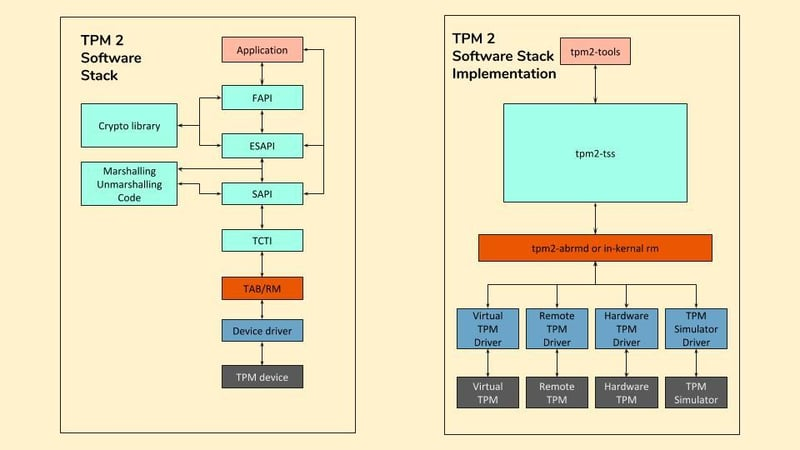
\includegraphics[width=0.77\textwidth]{figures/diagramma-tss-imp.png} % Inserisci qui il percorso della tua seconda immagine
    \caption{Diagramma \acrshort{tss} a sinistra e implementazione \texttt{tpm2-tools} a destra.}
    \label{fig:confronto_tss_tools}
\end{figure}

\texttt{tpm2-tools} è una suite potente ma presenta alcuni svantaggi che potrebbero limitarne l'uso in alcuni contesti. In primo luogo, essendo una suite a linea di comando, può risultare complessa per gli utenti che non sono familiari con i \textit{terminali} o con il funzionamento interno del \acrshort{tpm}.

Un altro aspetto limitante è che \texttt{tpm2-tools} opera principalmente a basso livello, il che significa che, per integrare il \acrshort{tpm} in applicazioni più complesse, potrebbe essere necessario scrivere codice aggiuntivo o fare affidamento su altre librerie. Questo lo rende meno adatto per chi cerca un'astrazione più alta e una soluzione pronta all'uso.

In termini di compatibilità, \texttt{tpm2-tools} è principalmente progettato per sistemi Linux, e potrebbe non essere ottimizzato o compatibile con altre piattaforme o dispositivi \acrshort{tpm}, limitandone l'utilizzo in ambienti eterogenei.

Un altro aspetto importante da considerare è che l'utilizzo di più strati di comunicazione nella suite può introdurre un certo \textit{overhead} di prestazioni, il che potrebbe essere problematico in ambienti dove è richiesta una gestione altamente performante delle risorse.

Infine, per sfruttare appieno le funzionalità di \texttt{tpm2-tools}, sono necessari strumenti esterni come il già citato \texttt{tpm2-abrmd}, che aggiungono un ulteriore livello di complessità alla configurazione e alla gestione del sistema.
\chapter{Applicazioni}\label{applicazioni}
\section{Measured Boot, Secure Boot e Trusted Boot}\label{sec:boot_types}

Nel paragrafo 1.2 Root of Trust si introduce il concetto di Root of Trust e le sue funzioni principali; tra questi ritroviamo il boot sicuro, descritto come l’instaurazione di una catena di fiducia necessaria per garantire un processo di avvio sicuro, garantire che il sistema sia in uno stato previsto (integrità della piattaforma) e rilevare eventuale codice manomesso. In altre parole, le \acrshort{rot} permettono a una piattaforma di dimostrare che è un ambiente affidabile.

All'accensione di un computer, il chip UEFI (che ha sostituito il tradizionale BIOS) viene eseguito per primo, ancora prima che qualsiasi altro componente entri in funzione. Il compito del UEFI è identificare l’hardware presente, configurarne il funzionamento, applicare le impostazioni correnti e determinare il dispositivo da cui eseguire l'avvio. Tuttavia, proprio perché questa fase precede l'attivazione di qualsiasi software di sicurezza e persino il caricamento del sistema operativo, rappresenta un momento vulnerabile in cui un hacker potrebbe iniettare codice malevolo per compromettere l'integrità del sistema. Per questo motivo, garantire che l’avvio della piattaforma avvenga in un ambiente sicuro e con codice affidabile è un requisito fondamentale per la protezione del sistema.

C’è molta confusione riguardo i concetti di Measured, Secured e Trusted boot, in questo capitolo si cerca di fare un po’ di chiarezza sui tre e su cosa li distingue uno dall’altro.

È essenziale tenere a mente che sono tre processi separati e differenti fra loro (soprattutto Measured e Secured). Il processo di avvio sicuro consolidato al momento, prevede che l’ordine di esecuzione delle tre fasi sia Measured Boot - Secure Boot - Trusted Boot. In realtà nessuna fase è obbligatoria, ma questo verrà esplorato più nel dettaglio nelle sezioni seguenti.

\subsection{Measured Boot}\label{subsec:measured_boot}

Il Measured Boot è un componente essenziale dell'architettura \acrshort{tpm} ed è alla base di molti altri meccanismi di sicurezza. Il suo scopo principale è garantire l’integrità dell’ambiente di pre-boot, ovvero la fase iniziale del processo di avvio, prima che il sistema operativo venga caricato. Il firmware e i bootloader del sistema utilizzano il \acrshort{tpm} per registrare e verificare che nessun componente sia stato alterato.

Questo processo si basa su una tecnica chiamata hash chaining, in cui ogni misurazione viene combinata con quella precedente attraverso un'operazione di hash extend (descritta nel capitolo 1.4.2.1). La specifica della piattaforma definisce quali \acrshort{pcr} devono essere utilizzati per ciascun componente del boot, e il primo codice eseguito –- che può essere il boot block del BIOS o l’intero firmware UEFI -– deve essere completamente protetto in scrittura. Questo impedisce a un attaccante di alterare il processo e registrare misurazioni false, preservando così l’attendibilità del sistema.

\begin{figure}[htbp]
    \centering
        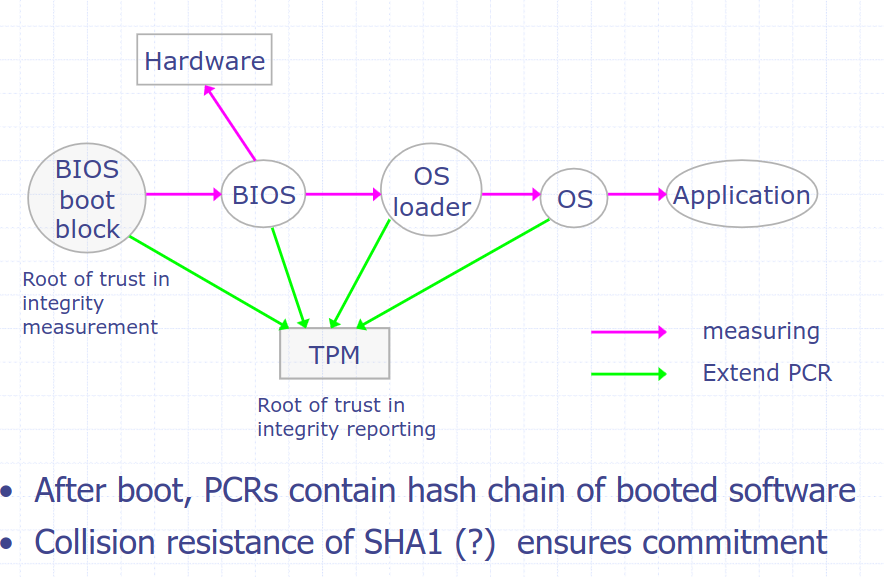
\includegraphics[width=0.77\textwidth]{figures/architettura-tcg.png}
    \caption{Slide dal corso sull’architettura \acrshort{tcg} della Stanford University.}
    \label{fig:architettura-tcg}
\end{figure}

Come conseguenza a questo processo, i \acrshort{pcr} conterranno la “hash-chain” calcolata su tutto il firmware, software e configurazioni della piattaforma.

UEFI inoltre abilita il Measured Boot a compiere un’operazione chiamata Remote Attestation che confronta le informazioni memorizzate nel \acrshort{tpm} con una versione sicura archiviata su un computer esterno, come un server aziendale o un servizio come Microsoft Endpoint Manager (InTune). Se i valori coincidono, significa che il \acrshort{tpm} non è stato alterato.

Nonostante la sua efficacia, Measured Boot is raramente utilizzato. La sua implementazione richiede un'infrastruttura complessa, con server di riferimento sicuri per la verifica, aumentando i costi e la difficoltà di gestione. Inoltre, la scarsa standardizzazione nell’uso dei \acrshort{pcr} e la compatibilità limitata con alcuni dispositivi e sistemi operativi ne ostacolano l'adozione. Soluzioni più semplici come Secure Boot e Trusted Boot sono spesso ritenute sufficienti, mentre Measured Boot resta principalmente una misura di sicurezza per ambienti ad alto rischio, come istituzioni governative o grandi enti finanziari.

\subsection{Secure Boot}\label{subsec:secure_boot}

Measured Boot conferma che il firmware e software non siano stati compromessi, quindi lo possiamo intuire come un controllo logico del codice e delle configurazioni della piattaforma. Il Secure Boot è invece un controllo hardware che assicura che il bootloader non sia stato manomesso. Fa parte dell'UEFI, un insieme di routine che forniscono le funzionalità di base per l'avvio del computer.

Secure Boot entra in gioco subito dopo l’avvio, o quando Measured Boot ha confermato con successo l'integrità del sistema se quest’ultimo è attivo. In pratica, verifica che tutto il codice eseguito prima del caricamento del sistema operativo sia affidabile: lo garantisce controllando che il firmware sia firmato digitalmente, riducendo il rischio di rootkit.

Solo il codice approvato dal produttore o dall'utente può essere eseguito. Se il bootloader o un altro componente non è firmato correttamente o non è riconosciuto dal produttore della scheda madre, come nel caso di software di terze parti, l'avvio viene impedito. Perseguendo gli obiettivi di una Root of Trust, Secure Boot permette di creare un percorso sicuro e affidabile che parte dall'UEFI e prosegue fino al kernel del sistema operativo.

È importante notare che, sebbene Secure Boot e Measured Boot condividano l'obiettivo di proteggere il sistema, differiscono nel modo in cui lo fanno. Secure Boot si limita a verificare la firma digitale del bootloader, mentre Measured Boot esegue un controllo più approfondito, registrando l'intero stato del software di avvio in modo verificabile successivamente. Tuttavia, il \acrshort{tpm} non impedisce direttamente l'avvio se rileva codice manomesso, il suo ruolo è solo quello di registrare i cambiamenti, lasciando ad altri meccanismi di sicurezza la decisione su come reagire. Solo Secure Boot ha la competenza di arrestare la sequenza d’avvio.

\subsection{Trusted Boot}\label{subsec:trusted_boot}

Se Secure Boot non rileva alcun problema e il processo di avvio prosegue, allora si attiva Trusted Boot, che effettua un ulteriore controllo per verificare che il bootloader, il kernel e altri componenti di basso livello non siano stati alterati dopo l’ultimo spegnimento del sistema. Trusted Boot è un meccanismo software che confronta il codice di avvio con i dati memorizzati nel \acrshort{tpm} durante l'ultimo arresto del sistema. Durante il Secure Boot il codice del \acrshort{so} non è disponibile, perché non è ancora stato caricato, mentre il Trusted Boot permette di verificare anche questi file.

Questa fase continua la chain of trust: il bootloader (verificato dal Secure Boot) verifica la firma digitale del kernel, mentre il kernel a sua volta controlla ogni altro componente dell’ambiente pre-boot del sistema operativo - inclusi i driver e i file di avvio. Come il Secure Boot, Trusted Boot è in grado di bloccare l’avvio di firmware o software modificato.

Per il \acrshort{tcg} il Trusted Boot è parte integrante della specifica, ma le implementazioni sono lasciate ai singoli sistemi operativi. Per le macchine che montano \acrshort{cpu} Intel-based il progetto di riferimento è tboot, un modulo open source che fa uso della tecnologia Intel Trusted Execution Technology. Per le piattaforme \acrshort{amd} il concetto è ripreso dalla tecnologia \acrshort{amd} Platform Security Processor. Una nota: l’azienda produttrice di \acrshort{amd} PSP ha rifiutato di rendere open source il progetto, suscitando critiche e accuse relative a possibili backdoor o meccanismi simili.

\section{Esempio di Measured Boot con Attestazione Remota}\label{sec:esempio_measured_boot}

Il sistema operativo Windows dalla versione 10 in poi, implementa tutti e tre i moduli Measure Boot (se il \acrshort{tpm} 2.0 è presente), Secure Boot e Trusted Boot -- sebbene siano tutti disattivabili dall’utente.

La minaccia principale da cui intende proteggere il \acrshort{pc} sono i rootkit, un tipo di malware sofisticato che opera in modalità kernel, utilizzando gli stessi privilegi del sistema operativo. Poiché i rootkit hanno gli stessi diritti del sistema operativo e si avviano prima di esso, possono nascondersi completamente agli occhi del \acrshort{so} o software anti-virus.

Nell’immagine di seguito (Figura 7) si osserva uno schema della chain of trust quando tutte e tre le fasi sono attive.

\begin{figure}[htbp]
    \centering
        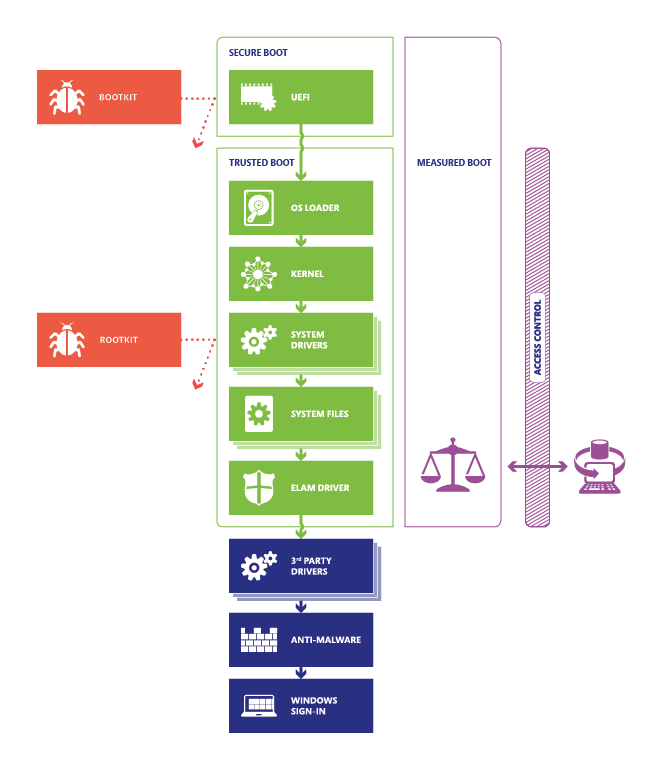
\includegraphics[width=0.8\textwidth]{figures/chain-of-trust.png}
    \caption{Processo di startup del sistema operativo Windows.
    }\label{fig:chain-of-trust}
\end{figure}

Un’aggiunta specifica dell’implementazione Microsoft è \acrfull{elam}, un modulo che interviene dopo la verifica del kernel da parte di Trusted Boot. Questo modulo testa i driver di avvio per verificare che tra questi non si nasconda del malware.

Measured Boot svolge il suo ruolo e le sue funzioni tradizionali come descritte nel capitolo 5.1.1, con la particolarità che necessita di una connessione ad un server di attestazione remoto per confermare le misurazioni \acrshort{tpm} ed i certificati sulla macchina locale.

In particolare l’implementazione di Windows segue questi passi:
\begin{itemize}
    \item Il firmware UEFI del \acrshort{pc} memorizza nel \acrshort{tpm} un hash del firmware, del bootloader, dei driver di avvio e di tutto ciò che viene caricato prima dell'app anti-malware.
    \item Al termine del processo di avvio, Windows avvia il client di attestazione remota. Il server invia al client una chiave unica.
    \item Il \acrshort{tpm} utilizza la chiave per firmare digitalmente il log registrato dall'UEFI.
    \item Il client invia il log al server, eventualmente insieme ad altre informazioni di sicurezza. A seconda dell'implementazione e della configurazione, il server può ora determinare se il client è sicuro.
\end{itemize}

\begin{figure}[htbp]
    \centering
    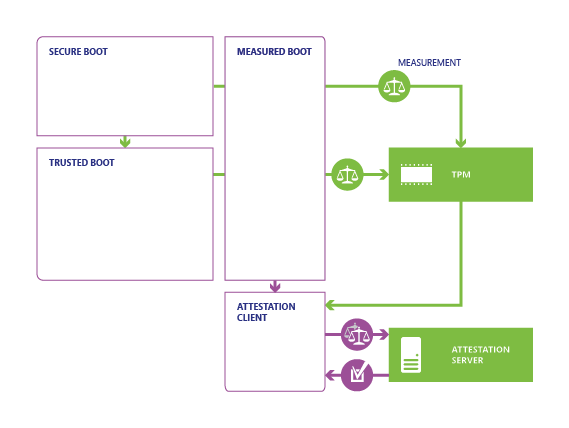
\includegraphics[width=0.5\textwidth]{figures/boot.png} 
    \caption{Attestazione Remota per il Measured Boot}\label{fig:remote_boot}
\end{figure}

Definiamo cosa si intende per Attestazione Remota (o Remote Attestation - RA): l'attestazione remota è un processo in cui una piattaforma fornisce prove verificabili sul suo stato di integrità a un verificatore remoto. Questo meccanismo consente di determinare se un sistema è sicuro senza la necessità di un'autorità di certificazione esterna, perché il verificatore può anche essere un server su cui sono depositati certificati o signatures digitali.

\section{BitLocker}\label{sec:bitlocker}

BitLocker è la funzionalità di crittografia completa del disco di Microsoft per Windows, introdotta in Windows Vista, progettata per proteggere i dati in caso di perdita, furto o smaltimento inappropriato del dispositivo. A partire da Windows 10 Versione 1511, BitLocker utilizza l'algoritmo di crittografia \acrshort{aes}-\acrshort{xts} per crittografare l'intero volume. Di default la chiave è di 128 bit ma è possibile usarne anche da 256 bit.

Il funzionamento di BitLocker si basa su una gerarchia di chiavi crittografiche. Alla base vi è la Full Volume Encryption Key (\acrshort{fvek}), utilizzata per crittografare l'intero disco e viene memorizzata nei metadati del disco in forma cifrata. La Volume Master Key (\acrshort{vmk}) protegge la \acrshort{fvek} ed è a sua volta crittografata tramite uno o più protector (protettori di chiave), come il Trusted Platform Module (\acrshort{tpm}), un \acrshort{pin} o una chiave USB.

Questo sistema a più livelli permette di cambiare le chiavi superiori senza dover decifrare e ri-cifrare l'intero volume, aumentando la flessibilità e la sicurezza del sistema. Quando una KPs è compromessa, vengono create nuove KPs e una nuova chiave principale del volume (\acrshort{vmk}), e la vecchia chiave di crittografia del volume completo (\acrshort{fvek}) viene crittografata con la nuova \acrshort{vmk}. In questo modo, anche se un attaccante ottiene la vecchia KPs, non può decifrare la \acrshort{fvek}.

\subsection{Processo di boot}\label{subsec:processo_de_boot}

BitLocker è generalmente integrato nel bootloader di Windows e viene eseguito prima della selezione del sistema operativo. Ma come fa Windows a riconoscere che il disco è crittografato?

Innanzitutto, BitLocker memorizza le informazioni relative alla crittografia del disco, inclusa l'eventuale presenza e posizione di una chiave. Durante il processo di avvio, diversi componenti del sistema, come il BIOS o UEFI, calcolano l'hash del proprio firmware e della configurazione, inviando poi tale valore al \acrshort{tpm}. Successivamente, il bootloader analizza i metadati del disco per determinare se sia crittografato. Se tutti i controlli sui file di avvio vengono superati, il sistema procede con l’esecuzione del kernel.

A questo punto, il kernel del sistema operativo inizializza le risorse necessarie e rileva l’unità crittografata. Tramite il \acrshort{tpm}, richiede l’accesso alla \acrshort{vmk}, necessaria per decrittografare la \acrshort{fvek} che poi viene utilizzata per decrittografare il contenuto del disco.

Infine, il kernel continua il processo di avvio decifrando ulteriori sezioni dell’unità man mano che diventano necessarie. In presenza del Trusted Boot, il kernel si occuperà anche di calcolare l’hash di alcuni file d’avvio e li invierà ai \acrshort{pcr}.

\subsection{Modalità di utilizzo}\label{subsec:modalita_di_utilizzo}

BitLocker offre tre modalità operative, delle quali le prime due richiedono la presenza di un modulo hardware per la crittografia, il \acrshort{tpm} versione 1.2 o successiva, e un firmware UEFI compatibile:
\begin{itemize}
    \item \textbf{Modalità Trasparente}: Questa modalità sfrutta le capacità del \acrshort{tpm} 1.2 per garantire un'esperienza utente senza interruzioni. La chiave di crittografia del disco viene memorizzata in forma crittografata all'interno del \acrshort{tpm}. Il caricatore del sistema operativo può accedere a questa chiave solo se i file di avvio risultano integri.
    \item \textbf{Modalità di Autenticazione Utente}: In questa modalità, l'utente è tenuto a inserire una chiave di autenticazione nell'ambiente pre-boot per poter avviare il sistema operativo. Sono supportati due metodi di autenticazione, tramite \acrshort{pin} (definito dall’utente) o chiave USB contenente la chiave di avvio necessaria per l'accesso al sistema.
    \item \textbf{Modalità Chiave USB (senza \acrshort{tpm})}: Questa modalità consente l'uso di BitLocker su sistemi privi di \acrshort{tpm}. È importante notare che questa modalità richiede che il BIOS o il firmware UEFI del sistema supporti la lettura dei dispositivi USB durante il processo di avvio. Inoltre, per il corretto funzionamento di BitLocker in questa configurazione, è necessario che il disco rigido sia formattato in almeno due volumi NTFS, uno di sistema e uno di avvio.
\end{itemize}

È fondamentale sottolineare che, nelle versioni client (ovvero non destinate ad un pubblico esperto) di Windows, solo il volume del sistema operativo può essere crittografato utilizzando BitLocker. Per la crittografia di dati sensibili in tempo reale su partizioni NTFS, si raccomanda l'uso del Encrypted File System (EFS), che può essere utilizzato in combinazione con BitLocker per una protezione aggiuntiva.

\subsection{Chiavi}\label{subsec:chiavi}

\textbf{STARTUP KEY}: L'amministratore del \acrshort{pc} crea una chiave di avvio durante l'inizializzazione di BitLocker. La chiave viene memorizzata su qualsiasi dispositivo di archiviazione come una chiavetta USB collegabile, e l'utente deve inserire tale dispositivo nel computer ogni volta che il computer viene avviato o riprende dallo stato di ibernazione. Mentre la chiavetta USB contenente la chiave di avvio deve essere collegata al computer dall'accensione fino al completamento dell'avvio, dovrebbe essere rimossa dopo il caricamento di Windows.

\textbf{RECOVERY KEY}: La chiave di ripristino può essere creata e salvata su una chiavetta USB durante la configurazione di BitLocker. Se il computer entra in modalità di ripristino, verrà richiesto all'utente di inserire la chiave di ripristino nel computer.

\textbf{CLEAR KEY}: se la verifica dell'integrità del sistema è disabilitata, la chiave principale di BitLocker è accessibile senza necessità di autenticazione. La sospensione di BitLocker cripta la chiave principale con una clear key, che è una chiave non protetta sul disco. Questo consente di apportare modifiche al sistema senza dover decifrare e ri-cifrare l'intero disco. Dopo le modifiche, quando BitLocker viene riattivato, quest'ultima sigilla nuovamente la chiave di crittografia con i nuovi valori dei componenti e cancella la clear key. Sebbene si tratti di una casistica che ricade nella manutenzione o quando si effettua un backup, dunque si tende ad eseguire queste operazioni in un ambiente sicuro e con tutte le precauzioni del caso, questa pseudo-esposizione della \acrshort{fvek} risulta una forte vulnerabilità in caso di attaccanti preparati.

\subsection{Critiche}\label{subsec:critiche}

Durante alcune operazioni di backup e ripristino, BitLocker non cifra i volumi finché l’utility di backup di Windows non riceve conferma dall’utente. Di conseguenza, i dati rimangono disponibili in chiaro durante la finestra temporale tra la preparazione del backup e la conferma. Questo consentirebbe ad un attaccante con accesso fisico di interrompere la decifratura automatica del disco durante un riavvio della macchina ed estrarre le chiavi. Sebbene si tratti di una casistica relativamente rara, Microsoft ha dichiarato che tale attacco è possibile solo quando BitLocker è configurato in modalità \acrshort{tpm}-only, che è la modalità predefinita. La configurazione di BitLocker con \acrshort{tpm}+\acrshort{pin}, invece, non è immediata e potrebbe risultare complessa per gli utenti meno esperti.

Nonostante Microsoft abbia negato la presenza di backdoor, la tecnologia supporta una "chiave di recupero" che potrebbe permettere l'accesso ai dati senza il consenso dell'utente, se questa chiave finisse nelle mani sbagliate.

Inoltre il fatto che il kernel venga caricato prima della vera e propria decifratura può rappresentare un ulteriore punto di vulnerabilità ad attacchi sofisticati che riescono a nascondersi e intercettare le chiavi crittografiche.

\subsection{Nota su \texorpdfstring{\acrshort{xts}}{XTS}}\label{subsec:nota_su_xts}

\acrshort{xts} è una soluzione di compromesso tra efficienza e sicurezza per la cifratura dei dischi, ma presenta limiti significativi che lo rendono inadatto come standard universale o per un utilizzo generalizzato e diffuso. La sua protezione è efficace solo quando il dispositivo è spento o bloccato, mentre a sistema acceso i dati rimangono accessibili, riducendo la sicurezza complessiva.

In un documento IEEE del 2007 viene segnalato che \acrshort{xts} è suscettibile alla manipolazione dei dati, poiché non prevede meccanismi di autenticazione: qualsiasi testo cifrato, anche se alterato da un attaccante, verrà comunque decifrato in un testo in chiaro senza alcun sistema integrato per rilevare modifiche o manomissioni. Per questo motivo, le applicazioni che richiedono una protezione più robusta devono adottare misure aggiuntive per verificare l’integrità dei dati e prevenire attacchi come la sostituzione di settori con versioni precedenti o la modifica di eseguibili.

Ulteriori critiche relative alla standardizzazione emergono anche da commenti pubblici su \acrshort{xts}-\acrshort{aes} richiesti dal NIST, successivi al documento IEEE del 2007.

Altri limiti di \acrshort{xts}-\acrshort{aes}: la sua struttura utilizza blocchi \acrshort{aes} da 16 byte, il che permette la manipolazione dei dati cifrati. Inoltre, presenta debolezze matematiche che consentono di recuperare il tweak principale in unità di dati grandi (ad esempio, su hard disk di grandi dimensioni). Inoltre, è vulnerabile ai timing attack.

Dal punto di vista tecnico, il riutilizzo delle chiavi su più blocchi e l'assenza di collegamento tra blocchi cifrati successivi espongono \acrshort{xts} a vulnerabilità come attacchi "taglia e incolla" e manipolazioni simili a quelle della modalità ECB, che può rivelare pattern nel testo cifrato. Di conseguenza, \acrshort{xts} è una soluzione di compromesso, adatta alla cifratura dei dischi, ma con limitazioni crittografiche rilevanti. Per mitigare queste debolezze, è fondamentale che le applicazioni implementino misure come l'uso di ridondanza nei testi in chiaro e il mantenimento di checksum per i dati, adottato nei file system come ZFS o Btrfs.

Per queste ragioni, \acrshort{xts} è considerabile al limite del compromesso accettabile. Alla luce delle criticità evidenziate da esperti nel settore, se \acrshort{xts}-\acrshort{aes} non è considerato idoneo per essere adottato come standard crittografico allora anche, la sua implementazione in sistemi ampiamente diffusi, come Windows, risulterebbe altamente sconsigliata. Questo è particolarmente rilevante considerando che la maggior parte degli utenti di tali sistemi non possiede le competenze necessarie per utilizzare consapevolmente questo strumento, aumentando così il rischio di un impiego non sicuro.

\subsection{Considerazioni}\label{subsec:considerazioni}

Nonostante le criticità progettuali, BitLocker, risi presenta come una soluzione adeguata per utenti non esperti e con esigenze di sicurezza limitate. BitLocker si avvale, infatti, di ulteriori misure di protezione, quali la verifica dell'integrità del bootloader e del kernel del sistema operativo. Pertanto, è raro che si verifichino le vulnerabilità discusse nelle sezioni precedenti, o, qualora si manifestino, sono generalmente presenti livelli di protezione superiori.

\subsection{Attacco BUS Sniff a BitLocker}\label{subsec:attacco_bus_sniff}

Un attacco recentemente dimostrato su un laptop ha consentito di estrarre la chiave di decrittazione di BitLocker in soli 43 secondi, utilizzando un Raspberry Pi Pico a basso costo. Questo exploit ha permesso di accedere e persino modificare i dati crittografati, mettendo in evidenza una vulnerabilità significativa.

Questo tipo di attacco non è una novità, in quanto Microsoft ne è a conoscenza e lo documenta nella sezione dedicata alle contromisure di BitLocker. L'azienda afferma che un attacco di questa natura richiede competenze avanzate, strumenti sofisticati e un accesso fisico prolungato. Ciò nonostante, la recente dimostrazione ha mostrato che, con una preparazione minima, è possibile eseguire l'attacco in meno di 50 secondi, utilizzando dispositivi economici e facilmente reperibili.

Durante l’avvio del sistema, i diversi componenti, come il BIOS/UEFI, eseguono una misurazione dell’integrità (come descritto nel capitolo 5.1). Se le misurazioni correnti corrispondono agli hash nei \acrshort{pcr}, allora il \acrshort{tpm} sblocca la chiave di BitLocker e la trasmette al processore.

Esiste, tuttavia, una vulnerabilità critica: la comunicazione tra il processore e il \acrshort{tpm} non è crittografata, e la chiave viene trasmessa in chiaro. Intercettando il traffico sul bus LPC (Low Pin Count), utilizzato da alcuni laptop per collegare il \acrshort{tpm} alla \acrshort{cpu}, è possibile estrarre la chiave di decrittazione. Per dimostrare tale vulnerabilità, è stato sviluppato un plugin per analizzatore logico, capace di monitorare il traffico su questo bus e di catturare la chiave di BitLocker.

Un attaccante, utilizzando un dispositivo basato su Raspberry Pi Pico, è riuscito a intercettare la comunicazione tra il \acrshort{tpm} e la \acrshort{cpu}, catturando la \acrshort{vmk} all'avvio del sistema. Con questa chiave, è possibile decrittografare l'SSD protetto da BitLocker usando un altra macchina con uno strumento come Dislocker, ottenendo accesso ai dati. Sebbene lo strumento sia stato progettato per un tipo specifico di laptop, non è inusuale trovare computer con un accesso simile ai pin del \acrshort{tpm}.

Questa dimostrazione evidenzia come, nonostante le misure di sicurezza di BitLocker, la protezione della chiave di decrittazione risulta vulnerabile se la comunicazione con il \acrshort{tpm} non è adeguatamente protetta.

\subsubsection{Mitigare l’attacco}\label{subsubsec:mitigare_attacco}

Alcune \acrshort{cpu} moderne sono dotate di f\acrshort{tpm} rendendo difficile intercettare il traffico sul bus -- anche se gli f\acrshort{tpm} non sono generalmente più sicuri dei d\acrshort{tpm}. Tuttavia, molti laptop aziendali continuano a utilizzare d\acrshort{tpm}, che sono vulnerabili ad attacchi sniff.

La configurazione di BitLocker che utilizza esclusivamente un \acrshort{tpm} è documentata come una delle soluzioni meno sicure. Sebbene questa configurazione offra una protezione relativamente solida contro l'accesso ai dati, tale protezione è efficace solo quando il disco è rimosso e separato sia dal sistema che dal \acrshort{tpm} stesso. In questa configurazione, esiste un unico ramo nella catena delle chiavi, dove il \acrshort{tpm} Key Protector decritta la \acrshort{vmk}, che a sua volta decritta la \acrshort{fvek}.

Microsoft suggerisce diverse misure di mitigazione, tra cui l'uso dell'autenticazione preboot con \acrshort{pin} associata al \acrshort{tpm}. Questa soluzione impedisce al \acrshort{tpm} di rilasciare automaticamente la chiave di BitLocker, introducendo un ulteriore livello di autenticazione. Il codice \acrshort{pin} richiesto all'avvio viene inserito prima che il \acrshort{tpm} possa sbloccare la \acrshort{vmk}. Tuttavia, la chiave rimane vulnerabile e può essere intercettata se un attaccante riesce a intercettare il traffico del bus nel momento esatto in cui il \acrshort{pin} viene inserito. Sebbene lo sniffing diventi tecnicamente più complesso la possibilità di un attacco non viene completamente eliminata.
\chapter{Altri approcci e prospettive}\label{approcci}

Nel capitolo 3.4 Variazioni del \acrshort{tpm} 2.0 viene proposta una panoramica sulle diverse forme che il \acrshort{tpm} può assumere. In questo capitolo verranno esplorate alcune soluzioni diverse dal tradizionale chip \acrshort{dtpm} saldato alla scheda madre di un \acrshort{pc}.

\section{\texorpdfstring{\acrshort{ftpm} e \acrshort{cpu} \acrshort{arm}}{fTPM e CPU ARM}}\label{sec:ftpm_cpu_arm}

Negli ultimi anni, le architetture \acrshort{cpu} commerciali come \acrshort{arm} e Intel hanno iniziato a integrare funzionalità per il calcolo sicuro. Queste tecnologie offrono ambienti di runtime isolati dal resto del software della piattaforma, inclusi sistema operativo, applicazioni e firmware. Tuttavia, presentano sfide significative poiché mancano di risorse sicure esterne alla \acrshort{cpu}, come l'archiviazione sicura e i contatori sicuri. 

\subsection{\texorpdfstring{\acrshort{arm} TrustZone}{ARM TrustZone}}\label{subsec:arm_trustzone}

\acrshort{arm} TrustZone è il supporto hardware di \acrshort{arm} per il calcolo sicuro, presente in molti recenti processori \acrshort{arm} (come Cortex A8, A9 e A15). Essa fornisce due processori virtuali, distinti tramite il controllo hardware dell'accesso. Il sistema software può passare tra due stati definiti "mondi": il Mondo Sicuro (\acrshort{sw}) e il Mondo Normale (\acrshort{nw}). Ogni mondo opera come un ambiente di runtime autonomo, con risorse proprie, come memoria, processore, cache, controller e interruzioni. Le risorse possono essere partizionate, condivise o riservate esclusivamente a uno dei mondi.

Come caratteristica architetturale, TrustZone non è un modulo software o hardware separato, ma una funzionalità integrata nell'architettura \acrshort{arm}. \acrshort{arm} progetta le \acrshort{cpu} e stabilisce le specifiche architetturali che i produttori di chip devono seguire, garantendo la conformità attraverso test di validazione. Ogni \acrshort{soc} \acrshort{arm} deve soddisfare questi standard per assicurare che TrustZone sia presente e funzionante.

Un importante vantaggio di questa implementazione è che la separazione tra il Mondo Sicuro (\acrshort{sw}) e il Mondo Normale (\acrshort{nw}) è garantita dall'hardware, evitando la dipendenza esclusiva da meccanismi software che potrebbero risultare vulnerabili a bug o exploit. Tuttavia, l'efficacia di questa protezione dipende dall'implementazione pratica adottata dai produttori di dispositivi.

Di seguito una panoramica delle funzionalità di \acrshort{arm} TrustZone.

\begin{itemize}
    \item \textbf{Secure Monitor}: \acrshort{arm} TrustZone crea due mondi separati, sicuro e non sicuro. Il monitor sicuro è una modalità del processore \acrshort{arm} che consente il passaggio di contesto tra il mondo sicuro e quello normale. Il processore \acrshort{arm} dispone di registri separati per ciascun mondo, con accesso limitato tra di essi. Un registro speciale stabilisce se il core esegue codice nel mondo sicuro o non sicuro, mentre il monitor sicuro consente il passaggio tra i mondi accedendo ai registri non sicuri. In modalità monitor, il processore è considerato sicuro, indipendentemente dal valore del registro.
    \item \textbf{Secure world entry/exit}: per design, una piattaforma \acrshort{arm} avvia sempre prima il mondo sicuro. In questa fase, il firmware di sistema può configurare l'ambiente di runtime del \acrshort{sw} prima che venga eseguito qualsiasi codice non verificato. Subito dopo il codice sicuro cede il controllo al mondo normale, dove può iniziare l'esecuzione di codice non affidabile. Il mondo normale utilizza l'istruzione \acrshort{arm} smc (secure monitor call) per trasferire il controllo al mondo sicuro attivando il monitor sicuro. Gli interrupt hardware possono essere indirizzati al monitor sicuro, permettendo una gestione flessibile e controllata degli interrupt.
    \item \textbf{Curtained Memory}: durante l'avvio, il software nel monitor sicuro può allocare una porzione di memoria esclusiva, chiamata memoria schermata, che non è accessibile al resto del sistema. \acrshort{arm} utilizza un segnale di controllo aggiuntivo (NS-bit, ad esempio il 33° bit su un architettura da 32 bit) per gestire l'accesso alla memoria: se il NS-bit è attivo, gli accessi alla memoria del mondo sicuro vengono bloccati.
\end{itemize}

\subsection{Problematiche e possibili soluzioni}\label{subsec:problematiche_soluzioni}

La specifica \acrshort{arm} TrustZone prevede protezione principalmente per la \acrshort{cpu}, i dispositivi \acrshort{io} e la memoria centrale. Poiché ogni produttore di \acrshort{soc} implementa TrustZone in modo diverso, esistono approcci variabili, ma alcune problematiche sono comuni tra i diversi produttori.

\begin{itemize}
    \item Mancanza di indicazioni per implementare uno spazio di archiviazione sicuro.
    \item Non è prevista una fonte sicura di entropia né un contatore persistente.
    \item La mancanza di obbligo nell'uso delle estensioni per la virtualizzazione \acrshort{arm} porta molti \acrshort{soc} mobili a non supportarla.
    \item La protezione di TrustZone non copre il bus periferico \acrshort{arm}, lasciando vulnerabili i sistemi sicuri a manipolazioni da parte del mondo non sicuro.
    \item Mancata concessione dell'accesso al firmware da parte dei fornitori di \acrshort{soc}. Si limita l'adozione di TrustZone per protegge la competitività.
\end{itemize}

Alcuni esperti hanno partecipato alla scrittura di un paper che propone un’implementazione di \acrshort{ftpm} in \acrshort{arm} TrustZone e rappresenta una buona base per un primo studio del caso d’uso. Per superare le limitazioni di \acrshort{arm} TrustZone, hanno adottato tre approcci: (1) fornire hardware di fiducia aggiuntivo, (2) fare compromessi di design che non compromettono la sicurezza del \acrshort{tpm}, e (3) modificare leggermente alcuni comandi \acrshort{tpm} 2.0 per adattarli alle limitazioni di TrustZone. Di seguito alcune delle proposte:

Al fine di lavorare su hardware fidato per garantire un livello minimo di supporto per \acrshort{ftpm}, sono stati introdotti requisiti hardware aggiuntivi . Il paper suggerisce di combinare partizioni \acrshort{rpmb} con la crittografia, ma non solo: si richiede la presenza di fuse hardware accessibili solo dal \acrshort{sw} (memoria impostata dai produttori con una chiave sicura unica) e una fonte di entropia accessibile dal \acrshort{sw}, che insieme alla chiave sicura viene utilizzata per generare chiavi crittografiche durante il boot. 

Per quanto riguarda la necessità di un clock sicuro, si sceglie di non prevedere hardware dedicato ma un meccanismo di timer sicuro che ticchetta ad un tasso pre-determinato.

I comandi long-running rappresentano un punto di instabilità per il \acrshort{tee}: primo fra tutti, la generazione di chiavi \acrshort{rsa}. La condivisione stabile del processore tra i due mondi dovrebbe essere fatta usando tecniche di virtualizzazione, ma molte piattaforme \acrshort{arm} mancano di supporto alla virtualizzazione. La soluzione diventa imporre che nessun percorso di codice \acrshort{tee} possa essere eseguito per lunghi periodi di tempo.

Viene anche affrontata la mancanza di archiviazione durante un periodo di "dark period" - periodi in cui i driver di archiviazione sicura non sono ancora caricati - modificando il \acrshort{tpm} 2.0 per interpretare diversamente il contatore dei tentativi falliti. Durante l'avvio, il \acrshort{ftpm} memorizza un "dirty bit". Se il \acrshort{ftpm} non riesce a salvare il bit, si blocca. Se durante il periodo di oscuramento (dark period) il sistema viene riavviato, e il "dirty bit" è attivo, il \acrshort{ftpm} considera un possibile attacco e incrementa il contatore dei tentativi falliti, mettendo il \acrshort{tpm} in modalità lockout. Un riavvio legittimo durante un "dark period" causa comunque l'ingresso del \acrshort{tpm} in modalità lockout, compromettendo l'usabilità. La specifica \acrshort{tpm} 2.0 include un "dirty bit", ma non prevede un numero limitato di tentativi prima del lockout, riducendo ulteriormente l'usabilità.

\subsection{Considerazioni}\label{subsec:considerazioni_ftpm}

Il paper mostra anche uno studio atto a rispondere a due domande sulla performance delle due forme di \acrshort{tpm}:
\begin{itemize}
    \item Qual è il sovraccarico dei comandi \acrshort{ftpm} a lungo termine, come la creazione di chiavi \acrshort{rsa}?
    \item Qual è il sovraccarico delle prestazioni dei comandi tipici dell'\acrshort{ftpm} e come si confronta con le prestazioni di un chip \acrshort{tpm} discreto?
\end{itemize}

Tutti i risultati evidenziano come gli \acrshort{ftpm} offrono prestazioni superiori rispetto ai \acrshort{tpm} discreti, con miglioramenti di performance che vanno da 2,4 a 15,12 volte. Il fatto non sorprende, poiché gli \acrshort{ftpm} eseguono il loro codice su processori \acrshort{arm} Cortex, mentre i chip discreti sono relegati all'uso di microprocessori molto più lenti. Le prestazioni degli \acrshort{ftpm} sembrano quindi essere vincolate principalmente dalla velocità del processore e dalla larghezza di banda della memoria.

Ad ogni modo l'argomento è complesso, e un singolo studio non è sufficiente a proporre un'architettura sicura alternativa. In particolare, lo studio analizzato in questo capitolo potrebbe non considerare appieno l'impatto in termini di usabilità dei dispositivi \acrshort{arm}, soprattutto riguardo ai compromessi e alle modifiche suggerite, che potrebbero risultare più evidenti sui dispositivi mobili rispetto agli \acrshort{soc} industriali.

Va inoltre nuovamente sottolineato che gli \acrshort{ftpm} non possono comunque fornire lo stesso grado di sicurezza di un dispositivo fisicamente dedicato come il \acrshort{dtpm}, ed inoltre sono particolarmente vulnerabili agli attacchi verso la memoria \acrshort{dram}. Sebbene entrambe le tecnologie siano suscettibili anche ai side attacks, la condivisione di risorse tra il mondo sicuro e quello normale costituisce sicuramente una base di attacco più ampia.

\section{\texorpdfstring{Intel \acrshort{txt} e \acrshort{amd} \acrshort{psp}}{Intel TXT e AMD PSP}}\label{sec:intel_txt_amd_psp}

Nel capitolo 5.1.3 Trusted Boot si menzionano due tecnologie, che stanno alla base delle implementazioni di Trusted Boot e sono impiegate per garantire sicurezza a livello hardware. Intel \acrshort{txt} e \acrshort{amd} \acrshort{psp} sono soluzioni progettate per proteggere l'integrità del sistema e dei dati, ma operano con approcci leggermente differenti - e sono previste per architetture hardware differenti.

\subsection{\texorpdfstring{Intel \acrshort{txt}}{Intel TXT}}\label{subsec:intel_txt}

Intel Trusted Execution Technology (\acrshort{txt}) è una tecnologia di sicurezza integrata nei processori Intel introdotta dal 2002. Si basa su una chain of trust che parte dall'hardware del microprocessore e si estende progressivamente. Dopo l'avvio, se l'utente desidera attivare la modalità sicura, viene eseguita una measured launch sequence (\acrshort{drtm}), che verifica l'integrità del sistema prima di consentire l'esecuzione del sistema operativo in un ambiente protetto. La sua função principale è la creazione di un Trusted Execution Environment (\acrshort{tee}) con l'obiettivo di proteggere il sistema da minacce come rootkit e malware.

Rispetto a una soluzione basata esclusivamente su \acrshort{tpm}, Intel \acrshort{txt} offre una Trusted Computing Base (\acrshort{tcb}) ridotta limitando il numero di componenti critici coinvolti nel processo di sicurezza. Due componenti fondamentali sono brevemente illustrati di seguito:

\begin{itemize}
    \item Il chipset contiene registri Intel \acrshort{txt} speciali, accessibili esclusivamente dal microcodice della \acrshort{cpu} o dagli Authenticated Code Modules (\acrshort{acm}s). Gli \acrshort{acm} sono moduli software firmati digitalmente da Intel eseguibili solo se autenticati tramite una chiave pubblica integrata nei registri hardware del chipset. Essi agiscono come estensioni del microcodice e operano in una memoria interna della \acrshort{cpu}, protetta da attacchi \acrshort{dma} e tecniche di snooping.
    \item Nello specifico, Intel \acrshort{txt} impiega due tipologie di \acrshort{acm}s: (1) BIOS \acrshort{acm}, responsabile dell’inizializzazione sicura del sistema e (2) SINIT \acrshort{acm}, attivato dal sistema operativo o da applicazioni per eseguire un measured launch attraverso la Dynamic Root of Trust for Measurement (\acrshort{drtm}), assicurando che il sistema venga eseguito solo in un ambiente verificato.
\end{itemize}

Intel \acrshort{txt} si integra strettamente con il \acrshort{tpm} 2.0, sfruttando registri e comandi dedicati. In particolare, utilizza i \acrshort{pcr} per il Measure Boot, registrando le misurazioni dei componenti coinvolti nel processo di avvio. Alcuni di questi registri possono essere estesi esclusivamente dal microcodice della \acrshort{cpu}, mentre altri sono modificabili solo dagli \acrshort{acm}s. Un altro oggetto \acrshort{tpm} soggetto della collaborazione sono gli indici \acrshort{nv}, che vengono impiegati per tracciare informazioni di stato. Oltre ai \acrshort{pcr}s e agli \acrshort{nv} indices, Intel \acrshort{txt} sfrutta comandi speciali del \acrshort{tpm} 2.0, tra cui comandi di policy e localities, per rafforzare i meccanismi di sicurezza.

Sebbene altre tecnologie Intel, come Boot Guard, utilizzino il \acrshort{tpm}, Intel \acrshort{txt} rappresenta l’esempio più diffuso di questa integrazione, soprattutto nelle piattaforme server.

\subsection{\texorpdfstring{\acrshort{amd} \acrshort{psp}}{AMD PSP}}\label{subsec:amd_psp}

\acrshort{amd} offre due opzioni ai produttori di piattaforme per integrare il \acrshort{tpm} nei loro sistemi: (1) \acrshort{dtpm} chip esterno tradizionale oppure (2) \acrshort{ftpm}. È una soluzione basata su software che viene eseguita all'interno del Platform Security Processor (\acrshort{psp}) di \acrshort{amd}. In questa configurazione, il \acrshort{tpm} è gestito tramite firmware, utilizzando il \acrshort{ccp} (Crypto Co-Processor) per l'elaborazione crittografica.

Il \acrshort{psp} è una tecnologia fondamentale integrata nei processori \acrshort{amd}, ma spesso rimane sconosciuta o ignorata dalla maggior parte degli utenti.

Il \acrshort{psp}, pur non influendo sull'uso quotidiano di un \acrshort{pc}, attira attenzione per la sua natura non documentata. Le suas potenti capacità di gestione della sicurezza gli consentono di accedere a dispositivi sulla Secure Memory Network (\acrshort{smn}) e alla memoria \acrshort{dram}, rendendolo un obiettivo interessante in caso di compromissione. Inoltre, può bypassare sistemi di sicurezza avanzati come la virtualizzazione sicura (\acrshort{sev}) o la sicurezza basata sulla virtualizzazione (\acrshort{vbs}).

\begin{figure}[htbp]
    \centering
        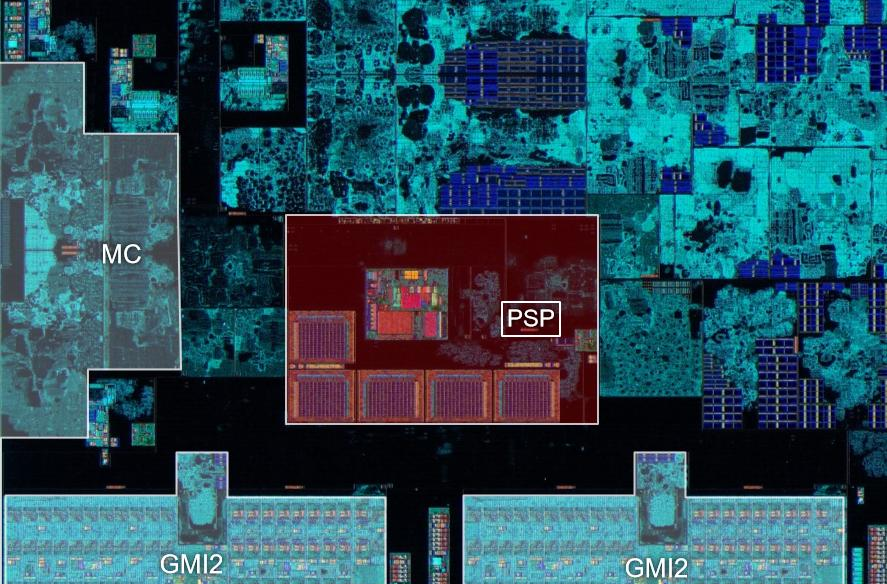
\includegraphics[width=0.9\textwidth]{figures/matisse-zen2.png}
    \caption{Fotografia di del chip \acrshort{amd} Matisse Zen2, con enfasi sul \acrshort{psp}. Crediti: Fritzchens Fritz.}
    \label{fig:matisse-zen2}
\end{figure}

Tali caratteristiche potrebbero sollevare preoccupazioni riguardo la possibile esposizione di chiavi e altre informazioni sensibili attraverso vulnerabilità come quelle scoperte in attacchi noti come quello del "glitch" PSPReverse. Nonostante queste potenzialità, la tecnologia \acrshort{psp} si distingue anche per la sua applicazione in ambito di protezione avanzata dei dati e di isolamento sicuro, ma la sua natura chiusa e la mancata documentazione sollevano interrogativi circa la trasparenza e il controllo su tali sistemi.

\subsection{Considerazioni}\label{subsec:considerazioni_txt_psp}

Sia Intel \acrshort{txt} che \acrshort{amd} \acrshort{psp} operano su principi simili, ovvero fornire una protezione a livello hardware contro la manipolazione del sistema e garantire che solo codice fidato venga eseguito. La differenza principale risiede nell'implementazione e nelle capacità specifiche di ciascuna piattaforma. Intel \acrshort{txt} si integra strettamente con il \acrshort{tpm} per misurare e validare l'integrità del sistema fin dall'avvio, mentre \acrshort{amd} \acrshort{psp} agisce come un'unità di sicurezza indipendente che gestisce in modo autonomo la protezione del sistema, senza fare affidamento diretto su un \acrshort{tpm}, ma su un’implementazione \acrshort{ftpm} propria.

Nel complesso, entrambe le tecnologie offrono solide basi per la creazione di sistemi sicuri. Queste tecnologie sono essenziali nell'evoluzione dei sistemi Trusted Processing Modules, poiché aumentano la resistenza contro minacce sia a livello di software che hardware.

\subsection{\texorpdfstring{\acrshort{amd} \acrshort{ftpm} stuttering}{AMD fTPM stuttering}}\label{subsec:amd_ftpm_stuttering}

Il problema di stuttering legato a \acrshort{ftpm} di \acrshort{amd} è stato rilevato per la prima volta su Windows nel 2022, quando gli utenti hanno notato blocchi casuali del sistema, non dipendenti dal carico di lavoro.

A partire dal kernel Linux 6.1, l'implementazione del \acrshort{ftpm} di \acrshort{amd} è stato abilitato per la generazione di numeri casuali tramite il modulo hardware \acrshort{rng}, impiegato per scopi di sicurezza. In particolare, quando un sistema è equipaggiato con un'unità \acrshort{ftpm} di \acrshort{amd}, il kernel utilizza automaticamente questa risorsa per gestire le operazioni che richiedono numeri casuali, con l'obiettivo di migliorare la sicurezza complessiva del sistema.

Tuttavia, questa implementazione ha causato problemi su alcune piattaforme, in particolare con processori \acrshort{amd} Ryzen, dove l’interazione tra \acrshort{ftpm} e il sistema di generazione dei numeri casuali ha provocato freeze intermittenti noti come stuttering, che si manifestavano in modo casuale durante l'utilizzo del computer. Questo comportamento è stato identificato come un bug legato al \acrshort{ftpm} e al modulo \acrshort{rng}.

Il rilascio di patch per risolvere il problema sono state precedute da accese discussioni nella comunità Linux. Nel luglio 2023, Linus Torvalds ha criticato aspramente l'implementazione, definendola "stupida" e suggerendo di disabilitarla per la generazione di numeri casuali. Una patch introdotta nel kernel 6.3 ha disabilitato \acrshort{ftpm} per l'\acrshort{rng} su sistemi problematici, ma il problema è riemerso anche con il kernel 6.4. La soluzione attuale prevede la disattivazione del supporto \acrshort{tpm} \acrshort{rng} per tutti i \acrshort{ftpm}, riducendo il problema senza eliminarlo completamente su alcune piattaforme.

Questo dibattito evidenzia le sfide nell'implementazione di soluzioni di sicurezza hardware e l'importanza di garantire che tali funzionalità non compromettano l'esperienza dell'utente finale.

\subsection{\texorpdfstring{Attacco faul\acrshort{tpm} \acrshort{amd}}{Attacco faulTPM AMD}}\label{subsec:attacco_faultpm_amd}

Un gruppo di ricercatori dell'Università Tecnica di Berlino ha recentemente individuato una vulnerabilità in alcune implementazioni \acrshort{ftpm}. Il loro studio dimostra come sia possibile compromettere \acrshort{psp} attraverso un attacco basato sull'iniezione di guasti (fault injection) tramite manipolazione della tensione in ingresso.

L’attacco sfrutta l'alterazione controllata della tensione di alimentazione del \acrshort{psp} all'interno delle architetture Zen 2 e Zen 3. Attraverso questa tecnica -- denominata faultTPM, i ricercatori sono riusciti a estrarre il "segreto" univoco di \acrshort{ftpm}, rendendo possibile la decodifica di tutti gli oggetti associati al modulo di sicurezza, e persino l’elusione di BitLocker di Windows.

Il team ha utilizzato strumenti economici e ha pubblicato sia codice che le specifiche dell’hardware impiegato su GitHub. L'attacco richiede ore di lavoro, accesso fisico al dispositivo e competenze avanzate, rendendolo difficile da eseguire su larga scala.

Nonostante la gravità della scoperta, il rischio per gli utenti è limitato, poiché l'attacco richiede accesso fisico. Tuttavia, una vulnerabilità così profonda solleva preoccupazioni significative. Rispetto ad altri attacchi side-channel, faultTPM rappresenta un avanzamento notevole, poiché consente di compromettere completamente il \acrshort{tpm} senza bypassare misure software complesse.

\acrshort{amd} non ha ancora rilasciato una soluzione definitiva, e il problema potrebbe non essere risolvibile con semplici aggiornamenti firmware. Possibili contromisure includono l'adozione di moduli \acrshort{tpm} hardware dedicati o una revisione architetturale. Al momento, gli utenti più esposti sono quelli che operano in ambienti ad alta sicurezza, dove l'accesso fisico ai dispositivi è una minaccia concreta.

\clearpage
\section{\texorpdfstring{Nota sull'\acrshort{iot}}{Nota sull'IoT}}\label{sec:nota_iot}

L’Internet of Things (\acrshort{iot}) ha portato a una crescente necessità di soluzioni di sicurezza integrate, poiché i dispositivi connessi operano spesso in ambienti esposti che necessitano di isolamento per le operazioni sensibili. In questo contesto, il Trusted Computing gioca un ruolo cruciale.

I \acrshort{tpm}, inizialmente sviluppati per i \acrshort{pc}, si stanno evolvendo per soddisfare le esigenze dei \acrshort{soc} e dei dispositivi embedded. Soluzioni integrate, come \acrshort{ftpm} e \acrshort{dtpm}, permettono di implementare funzionalità di sicurezza direttamente nei processori, riducendo l'esposizione dei bus di comunicazione e abbattendo i costi hardware.

Storicamente, i \acrshort{soc} \acrshort{arm} hanno trovato una maggiore diffusione nei dispositivi mobili, come smartphone e tablet, e, di conseguenza, i sistemi TrustZone non hanno generalmente impiegato un \acrshort{tpm} hardware separato. Considerando che il futuro dell'Internet of Things (\acrshort{iot}) sarà probabilmente dominato da architetture \acrshort{arm} anziché da x86 o x64, l'adoption di soluzioni basate su TrustZone potrebbe risultare ancora più rilevante per garantire la sicurezza e l'affidabilità dei dispositivi connessi. Tuttavia, è importante considerare che i controllori generalmente utilizzati nei sistemi \acrshort{iot} non possiedono elevate capacità prestazionali; pertanto, le funzionalità di sicurezza devono essere progettate in modo da non compromettere l'usabilità e la correttezza operativa del dispositivo.
\chapter*{Conclusione}\label{ch:conclusione}
\markboth{Conclusione}{Conclusione}
\addcontentsline{toc}{chapter}{Conclusione}

La rapida evoluzione e interconnessione della tecnologia ha reso la sicurezza informatica una delle priorità più urgenti. Questo vale anche e soprattutto in termini di privacy, un tema che accomuna utenti privati e istituzioni. Da un lato, gli utenti sono sempre più esposti a rischi che minano la privacy dei loro dati personali. Dall'altro, le istituzioni che gestiscono dati sensibili affrontano minacce complesse che potrebbero compromettere la riservatezza di informazioni strategiche, con impatti devastanti sia a livello economico che politico. Ma il nemico sta anche all’interno: è prioritario che le istituzioni o aziende che gestiscono, elaborano o memorizzano dati sensibili possano farlo in maniera trasparente, senza backdoor, senza possibilità di fughe di dati causate da malintenzionati infiltrati nell’entità stessa.

In tale contesto, il concetto di Trusted Computing si fa sempre più cruciale. Il \acrshort{tpm}, nato oltre vent’anni fa, ha rappresentato un pilastro fondamentale per la sicurezza informatica, garantendo operazioni sicure e la protezione dei dati sensibili in milioni di dispositivi. La sua implementazione ha permesso di costruire un’infrastruttura in cui ogni componente può fidarsi degli altri, riducendo il rischio di compromissione da parte di malware sofisticati. Da vent’anni di sviluppo si sono diffuse e discusse molte paure e diffidenze, specialmente per l'uso in ambienti \acrshort{pc}. Oggi questa tecnologia ha acquisito diversi gradi di maturità, e ormai lo standard dell’industria produce \acrshort{pc} già dotati di \acrshort{tpm}. 

Oggi il \acrshort{tpm} si sta evolvendo per affrontare le nuove sfide legate ai dispositivi embedded e all’\acrshort{iot}. L'adozione di \acrshort{tpm} in questi ambienti sta rapidamente crescendo, facendo emergere soluzioni che integrano la sicurezza direttamente nei processori e riducendo i rischi derivanti dalla trasmissione di dati sensibili.

Il prossimo obiettivo per l'elaborazione di informazioni affidabili riguarda, tra le altre, il campo dei sistemi embedded. Qual è lo standard, l'usabilità pratica e le vere problematiche in questo caso? Sebbene il \acrshort{tpm} abbia dimostrato la sua efficacia nel garantire la sicurezza nei personal computer, le sue applicazioni in ambienti diversi necessitano di adattamenti significativi. La realtà dell'\acrshort{iot} è profondamente diversa da quella dei \acrshort{pc} tradizionali: nei dispositivi \acrshort{iot}, le soluzioni di sicurezza devono essere progettate per trovare un giusto equilibrio tra prestazioni e costi, tenendo conto delle risorse limitate di questi dispositivi. Sebbene esistano soluzioni avanzate per proteggere i dati, esse spesso risultano troppo complesse o costose per essere implementate su larga scala in ambienti a bassa capacità. Di conseguenza, occorre affrontare la sfida di sviluppare soluzioni efficienti, scalabili e adeguate alle specifiche esigenze dei nuovi ambienti.

La sicurezza è sempre una catena e quello che conta è l'anello più debole.  Spesso questo anello è rappresentato dall'utente finale, infatti, la protezione offerta dai \acrshort{tpm} rischia di essere inefficace se non viene accompagnata da un'adeguata gestione della sicurezza a livello di interazione con l'utente ed egualmente di educazione informatica. Ma altrettanto frequentemente il punto di caduta può essere una svista progettuale, un piccolo dettaglio implementativo che, se avviene in ambito industriale o automotive, potrebbe risultare catastrofico.Oggi, il trusted computing si estende ben oltre i personal computer, interessando settori critici come la finanza, la sanità, l’industria e l’automotive. L’integrazione con nuove tecnologie, come l’Intelligenza Artificiale (\acrshort{ai}) e l’Internet of Things (\acrshort{iot}), evidenzia l’importanza di solide basi di sicurezza per proteggere infrastrutture sempre più complesse. Tuttavia sarà essenziale aggiornare costantemente gli standard di sicurezza e garantire che strumenti come il \acrshort{tpm}  rimangano efficaci nel tempo.

In un mondo digitale in continua evoluzione la fiducia non è solo un obiettivo, ma una necessità. Il Trusted Computing rappresenta una risposta solida e adattabile alle sfide della sicurezza informatica, fornendo una base essenziale per proteggere sistemi, dati e utenti anche nelle tecnologie di domani.
\begin{flushright}
    
\includegraphics[width=0.15\textwidth]{figures/firmetta.jpg}\label{fig:firmetta}
\end{flushright}

\chapter*{Appendice}\label{ch:appendix}
\markboth{Appendice}{Appendice}
\addcontentsline{toc}{chapter}{Appendice}

\begin{description}[itemsep=2.5ex, parsep=0.5ex, leftmargin=2.5cm, style=nextline]

    \item[\textbf{\acrshort{hsm}}] Con \acrshort{hsm} si intende Hardware Security Module, un dispositivo elaboratore fisico o una rete di dispositivi. Ha il compito di proteggere, gestire e scambiare chiavi digitali oltre che svolgere alcune operazioni crittografiche dedicate (come il calcolo hash per le firme digitali). Sono utilizzati in contesti di applicazioni di alto livello, come la gestione di chiavi per \acrshort{ssl}/\acrshort{tls} in server web, firma certificati in \acrshort{pki}, offload di operazioni crittografiche complesse in data center e generalmente hanno una maggiore capacità di calcolo dei \acrshort{pc} ordinari.

    \item[\textbf{\acrshort{tpm}}] Trusted Processing Module, il soggetto di questo testo. È uno standard internazionale riconosciuto come guida per la realizzazione di speciali microcontrollori dedicati a fornire un ancoraggio hardware sicuro. Il \acrshort{tpm} si interfaccia con il sistema informativo principale (solitamente un Personal Computer) fornendo operazioni che manipolano chiavi crittografiche in modo fidato e indipendente rispetto al software in esecuzione sul sistema.

    \item[\textbf{Secure Enclave}] Si intende la nozione di sistemi ideati per separare e proteggere l’esecuzione di codice e dati sensibili dal “resto del mondo”. Dove il “resto del mondo” è individuato come qualsiasi altro processo in esecuzione sul sistema - che sia eseguito in parallelo o in un altro momento.

    \item[\textbf{\acrshort{tee}}] Per esteso Trusted Execution Environment. Un \acrshort{tee} è un ambiente di esecuzione “fidato” - isolato - che garantisce la confidenzialità e integrità del codice e dati. 

    \item[\textbf{Piattaforma}] La macchina su cui è installato il \acrshort{tpm}.

    \item[\textbf{\acrshort{hmac}}] Un codice di autenticazione di messaggi basato su hash e chiave. Un uso importante degli \acrshort{hmac} nel \acrshort{tpm} è permettere ai processi utente di dimostrare la conoscenza di authdata. 

    \item[\textbf{BLOB}] Un oggetto binario di grandi dimensioni (Binary Large Object, blob) è un dato binario. Sebbene i dati possano avere significato per le applicazioni rilevanti, il termine blob enfatizza il trattamento dei dati come binari non strutturati che devono essere memorizzati o trasportati. Nel contesto del \acrshort{tpm}, i blob sono elementi di dati che l'utente è tenuto a memorizzare per conto del \acrshort{tpm} e a produrre quando necessario.

    \item[\textbf{\acrshort{srk}}] La Storage Root Key è la coppia di chiavi pubblica/privata alla radice della gerarchia delle chiavi di archiviazione del \acrshort{tpm}. 

    \item[\textbf{Authdata}] Password utilizzate per dimostrare di possedere l'autorizzazione ad utilizzare le risorse del \acrshort{tpm}, come le chiavi.

    \item[\textbf{\acrshort{pcr}}] Un Platform Configuration Register (\acrshort{pcr}) è un registro del \acrshort{tpm} che memorizza dati sulla configurazione della piattaforma, utilizzando "misurazioni" di hardware e software durante il processo di avvio. Il \acrshort{tpm} usa i \acrshort{pcr} per fornire garanzie sullo stato della piattaforma.

    \item[\textbf{Seal}] Nel contesto del \acrshort{tpm}, il "sealing" dei dati contro determinati valori di \acrshort{pcr} implica crittografare i dati in modo che il \acrshort{tpm} possa decifrarli se solo se i \acrshort{pcr} hanno i valori originali attesi. Questo può essere utilizzato per garantire l’accesso ai dati solo se la piattaforma si trova nello stato previsto.

    \item[\textbf{Messaggio}] Un array di byte scambiato tra due entità.

    \item[\textbf{Segretezza}] Un metodo per impedire a un osservatore non autorizzato di determinare il contenuto di un messaggio.

    \item[\textbf{Segreto condiviso}] Un valore noto a due parti. Il segreto può essere semplice come una password, oppure può essere una chiave di cifratura.

    \item[\textbf{Integrità}] La proprietà di un messaggio che non è stato alterato durante la memorizzazione o la trasmissione.

    \item[\textbf{Autenticazione}] Un metodo per indicare che un messaggio può essere legato al suo creatore, in modo che il destinatario possa verificar che solo il creatore avrebbe potuto inviare quel messaggio.

    \item[\textbf{Anti-ripetizione}] Un metodo per impedire a un attaccante di riutilizzare un messaggio valido (attacco replay).

    \item[\textbf{Non-ripudio}] Un metodo per impedire al mittente di un messaggio di affermare che non ha inviato il messaggio. È una proprietà molto forte.

    \item[\textbf{Autorizzazione}] Prova che l'utente è autorizzato a eseguire un'operazione o ad accedere a un'entità nel \acrshort{tpm}. 

    \item[\textbf{Sessione}] Come definito nella specifica \acrshort{tpm} 2.0, una "collezione di stato del \acrshort{tpm} che cambia dopo ogni utilizzo.". Le sessioni sono utilizzate per le autorizzazioni e per azioni di comando (crittografia, decrittografia, audit e alcune altre) in una sessione. Nel caso delle sessioni \acrshort{hmac} e di politica, le sessioni vengono create e poi utilizzate per più comandi. Le autorizzazioni tramite password sono un caso speciale di sessioni che non mantengono alcuno stato attraverso più comandi. I diversi tipi e utilizzi delle sessioni sono discussi ampiamente nei capitoli successivi; per ora è sufficiente avere una comprensione di alto livello.

    \item[\textbf{Handle}] Un identificatore che identifica in modo univoco una risorsa del \acrshort{tpm} che occupa la memoria del \acrshort{tpm}.

    \item[\textbf{Flusso di byte}] In un comando, i byte effettivi inviati al \acrshort{tpm}. In una risposta, i byte effettivi ricevuti dal \acrshort{tpm}.

    \item[\textbf{Dati canonicalizzati}] Le strutture C della specifica \acrshort{tpm} sono più grandi dei dati effettivamente trasmessi. Prima della trasmissione sono minimizzati per eliminare byte superflui. Questa ottimizzazione è essenziale dato che il \acrshort{tpm} usa bus lenti come LPC e SPI.

    \item[\textbf{\acrshort{tpme}}] Non è un termine ufficialmente definito nella specifica \acrshort{tcg}. In questo testo viene inteso come TPM Enablement, il meccanismo di abilitazione del \acrshort{tpm} che permette l’inizializzazione del \acrshort{tpm} e quindi la creazione dell’\acrshort{ek}.

    \item[\textbf{Locality}] Un meccanismo di sicurezza del \acrshort{tpm} 2.0 che consente di controllare l’accesso ai comandi e ai registri in base al livello di privilegio del software che li esegue.

\end{description}

% mostra tutte le citazioni anche se non sono state citate esplicitamente
%\nocite{*}
%\printbibliography[heading=bibintoc] % Bibliografia nell'indice

\chapter*{Ringraziamenti}\label{ch:ringraziamenti}
\markboth{Ringraziamenti}{Ringraziamenti}
\addcontentsline{toc}{chapter}{Ringraziamenti}

Ringrazio il Prof. Giuzzi che è stato il mio primo vero esame all'Università e che mi ha offerto di rifiutare un ventotto spaventandomi a morte per l'avvenire. Grazie per il supporto e l’opportunità che mi ha dato di scrivere una tesi su qualcosa che volevo davvero approfondire.

\end{document}